\documentclass[11pt,a4paper]{article}

% ===== FONT =====
\usepackage{iftex}
\ifPDFTeX
  \usepackage[T1]{fontenc}
  \usepackage[utf8]{inputenc}
  \usepackage[scaled=0.95]{helvet}
  \renewcommand{\familydefault}{\sfdefault}
\else
  \usepackage{fontspec}
  \defaultfontfeatures{Ligatures=TeX}
  \ifXeTeX
    \usepackage{polyglossia}
    \setdefaultlanguage{english}
  \fi
  \setmainfont{Helvetica}
  \setsansfont{Helvetica}
  \setmonofont{Menlo}
\fi
% ===== CORE PACKAGES =====
\usepackage{geometry}
\usepackage{microtype}
\usepackage{setspace}
\usepackage{enumitem}
\usepackage{float}
\usepackage{placeins}
\usepackage{graphicx}
\usepackage{caption}
\usepackage{capt-of} % for \captionof outside floats
\usepackage{subcaption}
\usepackage{multicol}
\usepackage{pifont}
\usepackage{adjustbox}

% ===== MATH =====
\usepackage{amsmath}
\let\Bbbk\relax
\usepackage{amssymb}
\usepackage{amsfonts}

% ===== TABLES =====
\usepackage{booktabs}
\usepackage{multirow}
\usepackage{array}
\usepackage{tabularx}
\usepackage{ragged2e}
\usepackage{siunitx}
\usepackage{colortbl}

% ===== STYLING & BOXES =====
\usepackage{xcolor}
\usepackage[most]{tcolorbox}
\usepackage{tikz}
\usetikzlibrary{shapes,arrows.meta,positioning,fit,backgrounds,calc,decorations.pathreplacing,chains}

% ===== HEADERS & SECTIONS =====
\usepackage{fancyhdr}
\usepackage{titlesec}
\usepackage{tocloft}

% ===== LINKS =====
\usepackage{hyperref}
\usepackage{xurl}
\usepackage{cleveref}
\usepackage[numbers,sort&compress]{natbib}

% ============================================================
% COLOR PALETTE
% ============================================================
\definecolor{velblue}{RGB}{22,58,108}
\definecolor{velaccent}{RGB}{70,98,146}
\definecolor{vellight}{RGB}{247,249,253}
\definecolor{velgold}{RGB}{164,123,66}
\definecolor{velgreen}{RGB}{60,112,82}
\definecolor{velred}{RGB}{146,68,68}
\definecolor{velorange}{RGB}{176,118,52}
\definecolor{velgray}{RGB}{248,249,252}
\definecolor{veldark}{RGB}{36,36,42}
\definecolor{rowalt}{RGB}{243,247,252}
\definecolor{rowhead}{RGB}{22,58,108}
\definecolor{tblhead}{RGB}{214,227,245}   % light blue-gray for header rows
\definecolor{velpenalty}{RGB}{150,82,82}
\definecolor{velok}{RGB}{58,108,78}
\definecolor{velhack}{RGB}{94,96,116}
\newcolumntype{Y}{>{\RaggedRight\arraybackslash}X}
\definecolor{velhacklight}{RGB}{248,248,250}

% ============================================================
% PAGE GEOMETRY
% ============================================================
\geometry{a4paper, left=0.70in, right=0.70in, top=0.72in, bottom=0.58in,
          headheight=12pt, headsep=14pt, footskip=26pt}
\setstretch{1.07}
\setlength{\parindent}{1.1em}
\setlength{\parskip}{0pt}
\setlength{\textfloatsep}{5pt plus 2pt minus 2pt}
\setlength{\floatsep}{5pt plus 2pt minus 2pt}
\setlength{\intextsep}{5pt plus 2pt minus 2pt}
\setlength{\emergencystretch}{2em}
\Urlmuskip=0mu plus 2mu
\hyphenation{or-ches-tra-tion com-pu-ta-tion ve-hi-cle het-er-o-ge-ne-ous meta-heu-ris-tic}
\graphicspath{{figures/}{images/}}
\raggedbottom
\captionsetup{font=small,labelfont=bf,skip=6pt}
\sisetup{detect-all,group-separator={,},group-minimum-digits=4}
\setlength{\tabcolsep}{8pt}
\renewcommand{\arraystretch}{1.22}

% ============================================================
% HYPERLINK SETUP
% ============================================================
\hypersetup{
    colorlinks=true, linkcolor=velblue, urlcolor=velaccent, citecolor=velblue,
    pdftitle={Velora Mobility Optimizer -- Technical Report},
    pdfauthor={Hostel ID: 2651},
}

% ============================================================
% SECTION FORMATTING
% ============================================================
\titleformat{\section}
  {\color{velblue}\normalfont\Large\bfseries}
  {\thesection}{0.8em}{}

\titleformat{\subsection}
  {\color{veldark}\normalfont\large\bfseries}
  {\thesubsection}{0.7em}{}

\titleformat{\subsubsection}
  {\color{velaccent}\normalfont\normalsize\bfseries}
  {\thesubsubsection}{0.6em}{}

\titlespacing*{\section}{0pt}{12pt}{6pt}
\titlespacing*{\subsection}{0pt}{9pt}{4pt}
\titlespacing*{\subsubsection}{0pt}{7pt}{3pt}

% ============================================================
% HEADER AND FOOTER
% ============================================================
\pagestyle{fancy}
\fancyhf{}
\renewcommand{\headrulewidth}{0.6pt}
\renewcommand{\headrule}{\vspace{-5pt}\hbox to\headwidth{\color{velblue}\leaders\hrule height \headrulewidth\hfill}}
\fancyhead[L]{\small\color{velblue}\textbf{Velora Mobility Optimizer}}
\fancyhead[R]{\small\color{velblue}Kriti '26 --- Technical Report}
\fancyfoot[C]{\small\thepage}

% ============================================================
% CALLOUT STYLES (academic, no dashboard cards)
% ============================================================
\newenvironment{callout}[1]{%
  \par\medskip
  \noindent\textbf{#1}\par
  \small\itshape
}{%
  \par\medskip\normalfont
}

% Backwards-compatible aliases (so existing content compiles)
\newenvironment{insightbox}[1][Discussion]{\begin{callout}{#1}}{\end{callout}}
\newenvironment{resultbox}[1][Result]{\begin{callout}{#1}}{\end{callout}}
\newenvironment{warnbox}[1][Constraint Note]{\begin{callout}{#1}}{\end{callout}}
\newenvironment{hackbox}[1][Hack Test Case]{\begin{callout}{#1}}{\end{callout}}
\newenvironment{phasebox}[2][]{\begin{callout}{#1}}{\end{callout}}

% ============================================================
% CUSTOM COMMANDS
% ============================================================
\newcommand{\rupee}{Rs.\,}
\newcommand{\statusok}{\textcolor{velok}{\textbf{\ding{51}~On-Time}}}
\newcommand{\statustol}{\textcolor{velorange}{\textbf{\ding{72}~Tolerance}}}
\newcommand{\statusviol}{\textcolor{velred}{\textbf{\ding{55}~Violated}}}
\newcommand{\cmark}{\textcolor{velok}{\ding{51}}}
\newcommand{\xmark}{\textcolor{velred}{\ding{55}}}
\newcommand{\saving}[1]{\textcolor{velok}{\textbf{#1}}}
\newcommand{\ph}[1]{\textbf{\textcolor{velaccent}{Phase #1}}}
\newcommand{\testcase}[3]{\subsection{#1 --- #2}\noindent #3\par\medskip}

% ---------- Test case layout helpers (prevent float drift) ----------
\newcommand{\TCSection}[2]{%
  \subsection{#1 --- #2}%
  \FloatBarrier
}
\newcommand{\TCTable}[2]{%
  \par\medskip
  \noindent\captionof{table}{#1}\par\vspace{4pt}%
  #2\par\medskip
}
\newcommand{\TCFigure}[3]{%
  \par\medskip
  \begin{center}
    \includegraphics[width=#1\linewidth]{#2}\par\vspace{2pt}
    \captionof{figure}{#3}%
  \end{center}
  \par\medskip
  \FloatBarrier
}

% Make existing \testcase use the pinned section macro
\renewcommand{\testcase}[3]{\TCSection{#1}{#2}\noindent #3\par\medskip}

% ============================================================
\begin{document}
% ============================================================

% ============================================================
% TITLE PAGE
% ============================================================
\begin{titlepage}
\thispagestyle{empty}
\centering

{\raggedleft
\includegraphics[height=2.42cm]{IITG.png}\par}
\vspace{0.3cm}
{\Large\bfseries End-Term Evaluation Submission\par}
\vspace{0.15cm}
{\normalsize 8th March 2026\par}

\vspace{0.15cm}

\includegraphics[width=0.46\linewidth]{Velora Logo.png}\par
\vspace{0.15cm}
{\LARGE\bfseries VELORA MOBITECH\par}

\vspace{0.45cm}
{\Large\bfseries Technical Report\par}
\vspace{0.1cm}
{\normalsize Kriti '26 --- Optimization Problem Statement\par}

\vspace{0.4cm}
\rule{0.86\linewidth}{0.6pt}\par
\vspace{0.35cm}

{\LARGE\bfseries Velora Mobility Optimizer\par}
\vspace{0.2cm}
{\itshape A Hybrid Metaheuristic Approach for the\par
Heterogeneous Vehicle Routing Problem\par
with Soft Time Windows (HVRPSTW)\par}

\vspace{0.35cm}
\rule{0.86\linewidth}{0.6pt}\par

\vspace{0.45cm}
\begin{tabular}{@{}rl@{}}
\textbf{Hostel ID:} & 2651 \\
\textbf{Submission Type:} & End Term Evaluation \\
\textbf{Problem Domain:} & Vehicle Routing Optimization \\
\textbf{Implementation:} & C++17 solver, Node.js backend, React frontend \\
\textbf{GitHub Repo:} & \href{https://github.com/bfea-kriti/VeloraMobilityOptimizer}{bfea-kriti/VeloraMobilityOptimizer} \\
\textbf{YouTube Demo:} & \href{https://www.youtube.com/watch?v=4BbK0500LLs}{Demonstration Video}\\
\end{tabular}

\vspace{0.4cm}
{\small
\href{https://velorafrontend-kri-2651-ti.onrender.com}{Frontend Deployment}
\quad|\quad
\href{https://velorabackend-kri-2651-ti.onrender.com}{Backend Deployment}
\quad|\quad
\href{https://github.com/bfea-kriti/VeloraMobilityOptimizer}{GitHub Repository}
\par}

\end{titlepage}

% ============================================================
% TABLE OF CONTENTS
% ============================================================
\renewcommand{\contentsname}{\Large\bfseries\color{velblue} Table of Contents}
\renewcommand{\cftsecfont}{\bfseries\color{velblue}}
\renewcommand{\cftsecpagefont}{\bfseries\color{velblue}}
\renewcommand{\cftsubsecfont}{\color{veldark}}
\setlength{\cftbeforesecskip}{4pt}
\setlength{\cftbeforesubsecskip}{1pt}
\renewcommand{\cftdotsep}{2}
\tableofcontents
\thispagestyle{fancy}
\newpage

% ============================================================
% SECTION 1: INTRODUCTION
% ============================================================
\section{Introduction}

Managing employee transportation is expensive and operationally complex. Every day, a company must decide which vehicle serves which employees, in what order, and at what time while balancing cost, capacity, time windows, vehicle types, and ride-sharing preferences. This is a vehicle-routing problem with heterogeneous fleets and service-quality constraints \cite{solomon1987,toth2014,laporte2009,purba2020}.

\textbf{Velora Mobility Optimizer} models this as a \textit{Heterogeneous Vehicle Routing Problem with Soft Time Windows} (HVRPSTW). Given a fleet and a set of pickup/dropoff requests, it computes routes that reduce transportation cost while enforcing hard constraints and pricing soft violations \cite{dondo2007,ismail2021}.

\subsection*{Problem Significance}
\begin{callout}{Why this problem matters}
In a city like Bengaluru, the per-employee per-day cab cost is roughly \textbf{\rupee 380--480}. For a 100-person team, that is over \textbf{\rupee 40,000 per day} and more than \textbf{\rupee 1 crore per year}. Shared routing can reduce that cost materially.
\end{callout}

\vspace{4pt}
\subsection*{System Overview}
The system is a full-stack web application:
\begin{itemize}[leftmargin=16pt,itemsep=2pt]
  \item \textbf{Solver:} C++17 binary implementing a 4-phase hybrid metaheuristic for heterogeneous fleet routing.
  \item \textbf{Backend:} Node.js/Express REST API that validates input, spawns the solver subprocess, and post-processes outputs.
  \item \textbf{Frontend:} React + Vite SPA with an interactive Leaflet map (OSRM road geometry), constraint analytics, and per-employee cost breakdowns.
  \item \textbf{Distance:} OSRM Table API for an NxN road-network distance matrix (with Haversine fallback); OSRM Route API for map visualization \cite{osrm2023}.
\end{itemize}

\subsection*{Hard vs. Soft Constraints}
\begin{center}
\small
\begin{tabularx}{0.96\textwidth}{@{}p{0.18\textwidth}XX@{}}
\toprule
\rowcolor{rowhead}\color{white}\textbf{Constraint} & \color{white}\textbf{Hard (always enforced)} & \color{white}\textbf{Soft (penalized)} \\
\midrule
\rowcolor{rowalt}Capacity   & Vehicle cannot exceed capacity  & --- \\
Precedence  & Pickup before dropoff (same req) & --- \\
\rowcolor{rowalt}Time Window & \small Pickup/drop beyond the hard deadline is an infeasible service event & \small Arrival within $[e_i, l_i + \delta_p]$ may incur penalty while still being tracked \\
Sharing     & ---                             & \small Max concurrent passengers; penalty per excess \\
\rowcolor{rowalt}Veh.\ Pref & ---                            & \small Employee's vehicle-type preference; penalty if unmet \\
\bottomrule
\end{tabularx}
\end{center}

\begin{insightbox}[Constraint Interpretation]
\small The implementation separates \textbf{soft lateness} from \textbf{hard infeasibility}. Service within the grace period is allowed with penalty; service beyond the hard deadline is treated as infeasible.
\end{insightbox}

% ============================================================
% SECTION 2: MATHEMATICAL FORMULATION
% ============================================================
\section{Mathematical Formulation}

We model employee transportation as a heterogeneous vehicle routing problem with soft time-window penalties on a directed graph
\[
G=(V,A), \qquad V=D\cup P\cup \{c\},
\]
where $D$ is the set of vehicle start depots, $P=\{1,\dots,n\}$ is the set of employee pickup requests, and $c$ is the common office node. Each request $i\in P$ corresponds to one pickup and one terminal drop at $c$. The formulation below captures the optimization structure solved approximately by the implemented hybrid metaheuristic \cite{golden2008,parragh2008,cordeau2001}.

\subsection{Sets, Parameters, and State Quantities}

For each vehicle $k\in K$, let $d(k)\in D$ be its start depot, $Q_k$ its capacity, $C_k$ its cost per kilometre, and $A_k$ its earliest departure time. For each arc $(u,v)\in A$, let $d_{uv}$ and $\tau_{uv}$ denote travel distance and travel time, respectively. For each request $i\in P$, let $[E_i,L_i]$ denote the preferred service interval, let $\delta_i=f(P_i)$ denote the priority-based tolerance beyond $L_i$, let $\omega_i=6-P_i$ be the priority weight, let $h_i$ be the sharing limit, let $\gamma_i$ denote the preferred vehicle class, and let
\[
K_i^{\mathrm{pref}}=\{k\in K:\text{vehicle }k\text{ satisfies }\gamma_i\}.
\]
The tolerance function used in the solver is
\[
f(1)=5,\qquad f(2)=10,\qquad f(3)=15,\qquad f(4)=20,\qquad f(5)=30,
\]
measured in minutes. The severe violation multiplier is fixed at $M=1000.0$.

\subsection{Decision Variables}

The routing and service decisions are represented by:
\begin{align}
x_{uv}^k &\in \{0,1\} && \text{1 if vehicle $k$ traverses arc $(u,v)$,} \\
y_i^k &\in \{0,1\} && \text{1 if request $i$ is assigned to vehicle $k$,} \\
z_i &\in \{0,1\} && \text{1 if request $i$ is left unassigned,} \\
t_u^k &\ge 0 && \text{arrival time of vehicle $k$ at node $u$,} \\
q_u^k &\ge 0 && \text{load of vehicle $k$ after leaving node $u$.}
\end{align}

Penalty quantities are accumulated through auxiliary variables:
\begin{align}
\ell_i &\ge 0 && \text{hard-constraint excess beyond }L_i+\delta_i, \\
s_i &\ge 0 && \text{sharing-limit excess for request }i, \\
p_i &\in \{0,1\} && \text{vehicle-preference violation indicator.}
\end{align}

\subsection{Objective Function}

The objective combines transport cost, route duration, and service-quality penalties:
\begin{equation}
\min F =
w_c \sum_{k\in K}\sum_{(u,v)\in A} C_k d_{uv}x_{uv}^k
\, + \,
w_t \sum_{k\in K}\sum_{(u,v)\in A} \tau_{uv}x_{uv}^k
\, + \,
M\sum_{i\in P}\omega_i \ell_i
\, + \,
\lambda_s\sum_{i\in P}s_i
\, + \,
\lambda_p\sum_{i\in P}p_i
\, + \,
\lambda_u\sum_{i\in P}z_i .
\label{eq:objective-full}
\end{equation}

Equation~\eqref{eq:objective-full} is a business objective, not a pure distance minimizer. It combines transport cost, route duration, hard time-window violations, service-quality penalties, and unserved demand.

\subsection{Core Constraints}

\subsubsection{Assignment and Visit Consistency}
Each request is either assigned to exactly one vehicle or marked unassigned:
\begin{equation}
\sum_{k\in K} y_i^k + z_i = 1
\qquad \forall i\in P .
\label{eq:assign}
\end{equation}
If request $i$ is assigned to vehicle $k$, then that vehicle must enter and leave the pickup node exactly once:
\begin{equation}
\sum_{u\in V} x_{ui}^k = y_i^k,
\qquad
\sum_{v\in V} x_{iv}^k = y_i^k
\qquad \forall i\in P,\ \forall k\in K .
\label{eq:visit-link}
\end{equation}

\subsubsection{Route Initiation and Flow Conservation}
Each vehicle starts from its own depot and, if used, terminates at the common office node:
\begin{equation}
\sum_{v\in V} x_{d(k)v}^k
=
\sum_{u\in V} x_{uc}^k
\le 1
\qquad \forall k\in K .
\label{eq:start-end}
\end{equation}
For intermediate nodes, incoming and outgoing flow must balance:
\begin{equation}
\sum_{v\in V} x_{uv}^k - \sum_{v\in V} x_{vu}^k = 0
\qquad \forall u\in V\setminus\{d(k),c\},\ \forall k\in K .
\label{eq:flow}
\end{equation}

\subsubsection{Temporal Feasibility}
Arrival times propagate along active arcs through the standard big-$M$ relation
\begin{equation}
t_v^k \ge t_u^k + \tau_{uv} - M(1-x_{uv}^k)
\qquad \forall (u,v)\in A,\ \forall k\in K ,
\label{eq:time-prop}
\end{equation}
with depot availability
\begin{equation}
t_{d(k)}^k \ge A_k
\qquad \forall k\in K .
\label{eq:depot-start}
\end{equation}

\subsubsection{Lateness Penalty (Two-Tier Structure)}
For each employee $i$, let $t_c^k$ denote the arrival time at the office (drop-off node $c$) by the assigned vehicle $k$. Let $\delta_i=f(P_i)$ denote the priority-based tolerance. The penalty is
\begin{equation}
\mathrm{Penalty}_i=
\begin{cases}
0, & \text{if } t_c^k \le L_i+\delta_i \quad \text{(on-time or within tolerance)}, \\[4pt]
(t_c^k-L_i-\delta_i)\,M\,\omega_i, & \text{if } t_c^k > L_i+\delta_i \quad \text{(exceeds tolerance)} .
\end{cases}
\label{eq:two-tier-penalty}
\end{equation}
where:
\begin{itemize}[leftmargin=16pt,itemsep=2pt]
  \item $L_i$ is the latest acceptable drop-off time for employee $i$.
  \item $\delta_i=f(P_i)$ is the priority-based tolerance, with $f(1)=5$, $f(2)=10$, $f(3)=15$, $f(4)=20$, and $f(5)=30$ minutes.
  \item $M=1000.0$ is the severe violation penalty multiplier.
  \item $\omega_i = 6-P_i$ is the priority weight.
\end{itemize}
Equivalently, the violation magnitude recorded in the optimization model is
\begin{equation}
\ell_i \ge t_c^k-(L_i+\delta_i)-M(1-y_i^k)
\qquad \forall i\in P,\ \forall k\in K .
\label{eq:lateness}
\end{equation}
\noindent\textbf{Key insight:} No penalty is applied if the employee arrives by $L_i+\delta_i$. Only later arrivals trigger the severe violation term.

\subsubsection{Capacity Feasibility}
Because every route accumulates pickups before reaching the common office node, onboard load is nondecreasing until termination. The load evolution is therefore bounded by
\begin{equation}
q_v^k \ge q_u^k + y_v^k - M(1-x_{uv}^k)
\qquad \forall u\in V,\ \forall v\in P,\ \forall k\in K ,
\label{eq:load-prop}
\end{equation}
together with
\begin{equation}
0 \le q_u^k \le Q_k
\qquad \forall u\in V,\ \forall k\in K .
\label{eq:capacity}
\end{equation}

\subsubsection{Soft Preference Variables}
The remaining service-quality quantities are modeled as
\begin{align}
s_i &\ge b_i-h_i, \qquad s_i \ge 0 && \forall i\in P , \label{eq:sharing-slack}\\
p_i &\ge 1-\sum_{k\in K_i^{\mathrm{pref}}} y_i^k && \forall i\in P , \label{eq:pref-slack}
\end{align}
where $b_i$ denotes the maximum concurrent onboard load experienced by request $i$ along its assigned route. Thus, $s_i$ measures the amount by which the sharing limit is exceeded, and $p_i$ activates whenever the assigned vehicle does not belong to the preferred class set.

\FloatBarrier
% ============================================================
% SECTION 3: SYSTEM ARCHITECTURE AND DEPLOYMENT
% ============================================================
\section{System Architecture and Deployment}
\label{sec:architecture}

Velora Mobility Optimizer follows a four-layer pipeline: frontend, backend, parser, and C++ solver. The frontend collects input files and renders outputs, the backend validates requests and launches the solver, the parser normalizes spreadsheet data, and the solver writes route JSON and summary metrics.

\begin{figure}[H]
\centering
\resizebox{0.95\linewidth}{!}{%
\begin{tikzpicture}[
  font=\footnotesize,
  arrow/.style={->, line width=0.8pt, >=Stealth, draw=velhack},
  box/.style={rectangle, draw=velhack, rounded corners=3pt,
              fill=vellight, line width=0.6pt,
              inner sep=6pt, align=left, text width=4.35cm,
              minimum height=1.9cm},
  tag/.style={font=\scriptsize\bfseries, text=velblue}
]

% --- Row 1 ---
\node[box] (s1) {\textbf{1. Data ingestion}\par
\small Upload Excel/JSON\par Fleet + requests\par Start workflow};
\node[box, right=6mm of s1] (s2) {\textbf{2. Parse request}\par
\small Frontend uploads file\par Multer stores upload\par Backend triggers parser};
\node[box, right=6mm of s2] (s3) {\textbf{3. Excel $\to$ JSON}\par
\small \texttt{excel\_to\_json.py}\par Read vehicles/employees\par Normalize windows};
\vspace{8pt}
% --- Row 2 ---
\node[box, below=7mm of s1] (s4) {\textbf{4. Preview UI}\par
\small Validate inputs\par Show parsed preview\par Enable optimize};
\node[box, right=6mm of s4] (s5) {\textbf{5. Optimize trigger}\par
\small POST \texttt{/api/optimize}\par Weights + penalties\par Budget included};
\node[box, right=6mm of s5] (s6) {\textbf{6. Input preparation}\par
\small Backend validation\par Normalize fields\par Write input JSON};
\vspace{8pt}
% --- Row 3 ---
\node[box, below=7mm of s4] (s7) {\textbf{7. C++ optimizer}\par
\small \texttt{velora\_solver}\par 4-phase metaheuristic\par Distance matrix};
\node[box, right=6mm of s7] (s8) {\textbf{8. Solver output}\par
\small Route JSON on disk\par Convergence log/CSV\par Unassigned tracked};
\node[box, right=6mm of s8] (s9) {\textbf{9. Post-processing}\par
\small Summary metrics\par Constraint analysis\par Enrichment};
\node[box, right=6mm of s9] (s10) {\textbf{10. Results delivery}\par
\small Dashboard + maps\par Exports (JSON/Excel/PDF)\par Client display};

% --- Arrows ---
\draw[arrow] (s1) -- (s2);
\draw[arrow] (s2) -- (s3);
\draw[arrow] (s3.south) -- ++(0,-4mm) -| (s4.north);
\draw[arrow] (s4) -- (s5);
\draw[arrow] (s5) -- (s6);
\draw[arrow] (s6.south) -- ++(0,-4mm) -| (s7.north);
\draw[arrow] (s7) -- (s8);
\draw[arrow] (s8) -- (s9);
\draw[arrow] (s9) -- (s10);

% --- Section tags ---
\node[tag] at ($(s1.north)!0.5!(s3.north) + (0,3mm)$) {FRONTEND + INGEST};
\node[tag] at ($(s4.north)!0.5!(s6.north) + (0,3mm)$) {API ORCHESTRATION};
\node[tag] at ($(s7.north)!0.5!(s10.north) + (0,3mm)$) {OPTIMIZATION CORE};

\end{tikzpicture}}
\caption{Execution pipeline from file upload to result delivery.}
\label{fig:dataflow-10stage}
\end{figure}

\begin{figure}[H]
\centering
\resizebox{0.94\linewidth}{!}{%
\begin{tikzpicture}[
  font=\footnotesize,
  arrow/.style={->, line width=0.8pt, >=Stealth, draw=velhack},
  box/.style={rectangle, draw=velhack, rounded corners=3pt,
              fill=vellight, line width=0.6pt,
              inner sep=6pt, align=left},
  lbl/.style={font=\scriptsize, text=veldark}
]

% --- Top row: USER -> FRONTEND -> BACKEND ---
\node[box, text width=2.8cm, minimum height=1.25cm] (user) {%
\textbf{User}\par\small Web browser};

\node[box, right=12mm of user, text width=3.8cm, minimum height=1.55cm] (frontend) {%
\textbf{Frontend}\par\small React + Vite\par\small Port 5173\par\small Dashboard + map};

\node[box, right=12mm of frontend, text width=4.0cm, minimum height=1.55cm] (backend) {%
\textbf{Backend}\par\small Express.js API\par\small Port 3001\par\small Validation + orchestration};

% --- Second row: Inputs, Solver, JSON, Reports ---
\node[box, below=12mm of user, text width=2.8cm, minimum height=1.15cm] (inputs) {%
\textbf{Excel / JSON}\par\small Inputs};

\node[box, below=12mm of backend, xshift=-2.2cm, text width=3.8cm, minimum height=1.45cm] (solver) {%
\textbf{Solver}\par\small C++17 engine\par\small SA + ALNS + heuristics};

\node[box, right=12mm of solver, text width=2.8cm, minimum height=1.15cm] (json) {%
\textbf{JSON}\par\small Prepared I/O};

\node[box, right=12mm of json, text width=2.8cm, minimum height=1.15cm] (reports) {%
\textbf{Reports}\par\small Metrics + exports};

% --- Arrows ---
\draw[arrow] (user)     -- node[above, lbl] {HTTP}     (frontend);
\draw[arrow] (frontend) -- node[above, lbl] {REST API}  (backend);
\draw[arrow] (inputs)   -- node[above, lbl] {upload}    (frontend.south west);
\draw[arrow] (backend.south) -- ++(0,-4mm) -| node[pos=0.25, right, lbl] {subprocess} (solver.north);
\draw[arrow] (solver.east) -- (json.west);
\draw[arrow] (json.north) -- ++(0,4mm) -| (backend.south);
\draw[arrow] (json)     -- (reports);

\end{tikzpicture}}
\caption{Layered architecture and artifact flow.}
\label{fig:full-arch}
\end{figure}

\subsection{Deployment}

Both web services are hosted on \textbf{Render}; the backend runs the solver as a subprocess and returns JSON results to the frontend.

\begin{center}
\small
\begin{tabularx}{0.82\linewidth}{@{}p{0.30\linewidth}X@{}}
\toprule
\rowcolor{rowhead}\color{white}\textbf{Surface} & \color{white}\textbf{Link} \\
\midrule
\rowcolor{rowalt}Frontend &
\href{https://velorafrontend-kri-2651-ti.onrender.com}{velorafrontend-kri-2651-ti.onrender.com} \\
Backend API &
\href{https://velorabackend-kri-2651-ti.onrender.com}{velorabackend-kri-2651-ti.onrender.com} \\
\rowcolor{rowalt}GitHub Repository &
\href{https://github.com/bfea-kriti/VeloraMobilityOptimizer}{github.com/bfea-kriti/VeloraMobilityOptimizer} \\
Demonstration Video &
\href{https://www.youtube.com/watch?v=4BbK0500LLs}{youtube.com/watch?v=4BbK0500LLs} \\
\bottomrule
\end{tabularx}
\end{center}

\noindent The frontend handles upload, validation, and result inspection. The backend handles preprocessing, solver orchestration, and exports.

\begin{figure}[H]
\centering
\makebox[\linewidth][c]{%
\subcaptionbox{Upload and runtime controls\label{fig:ui-upload}}{%
  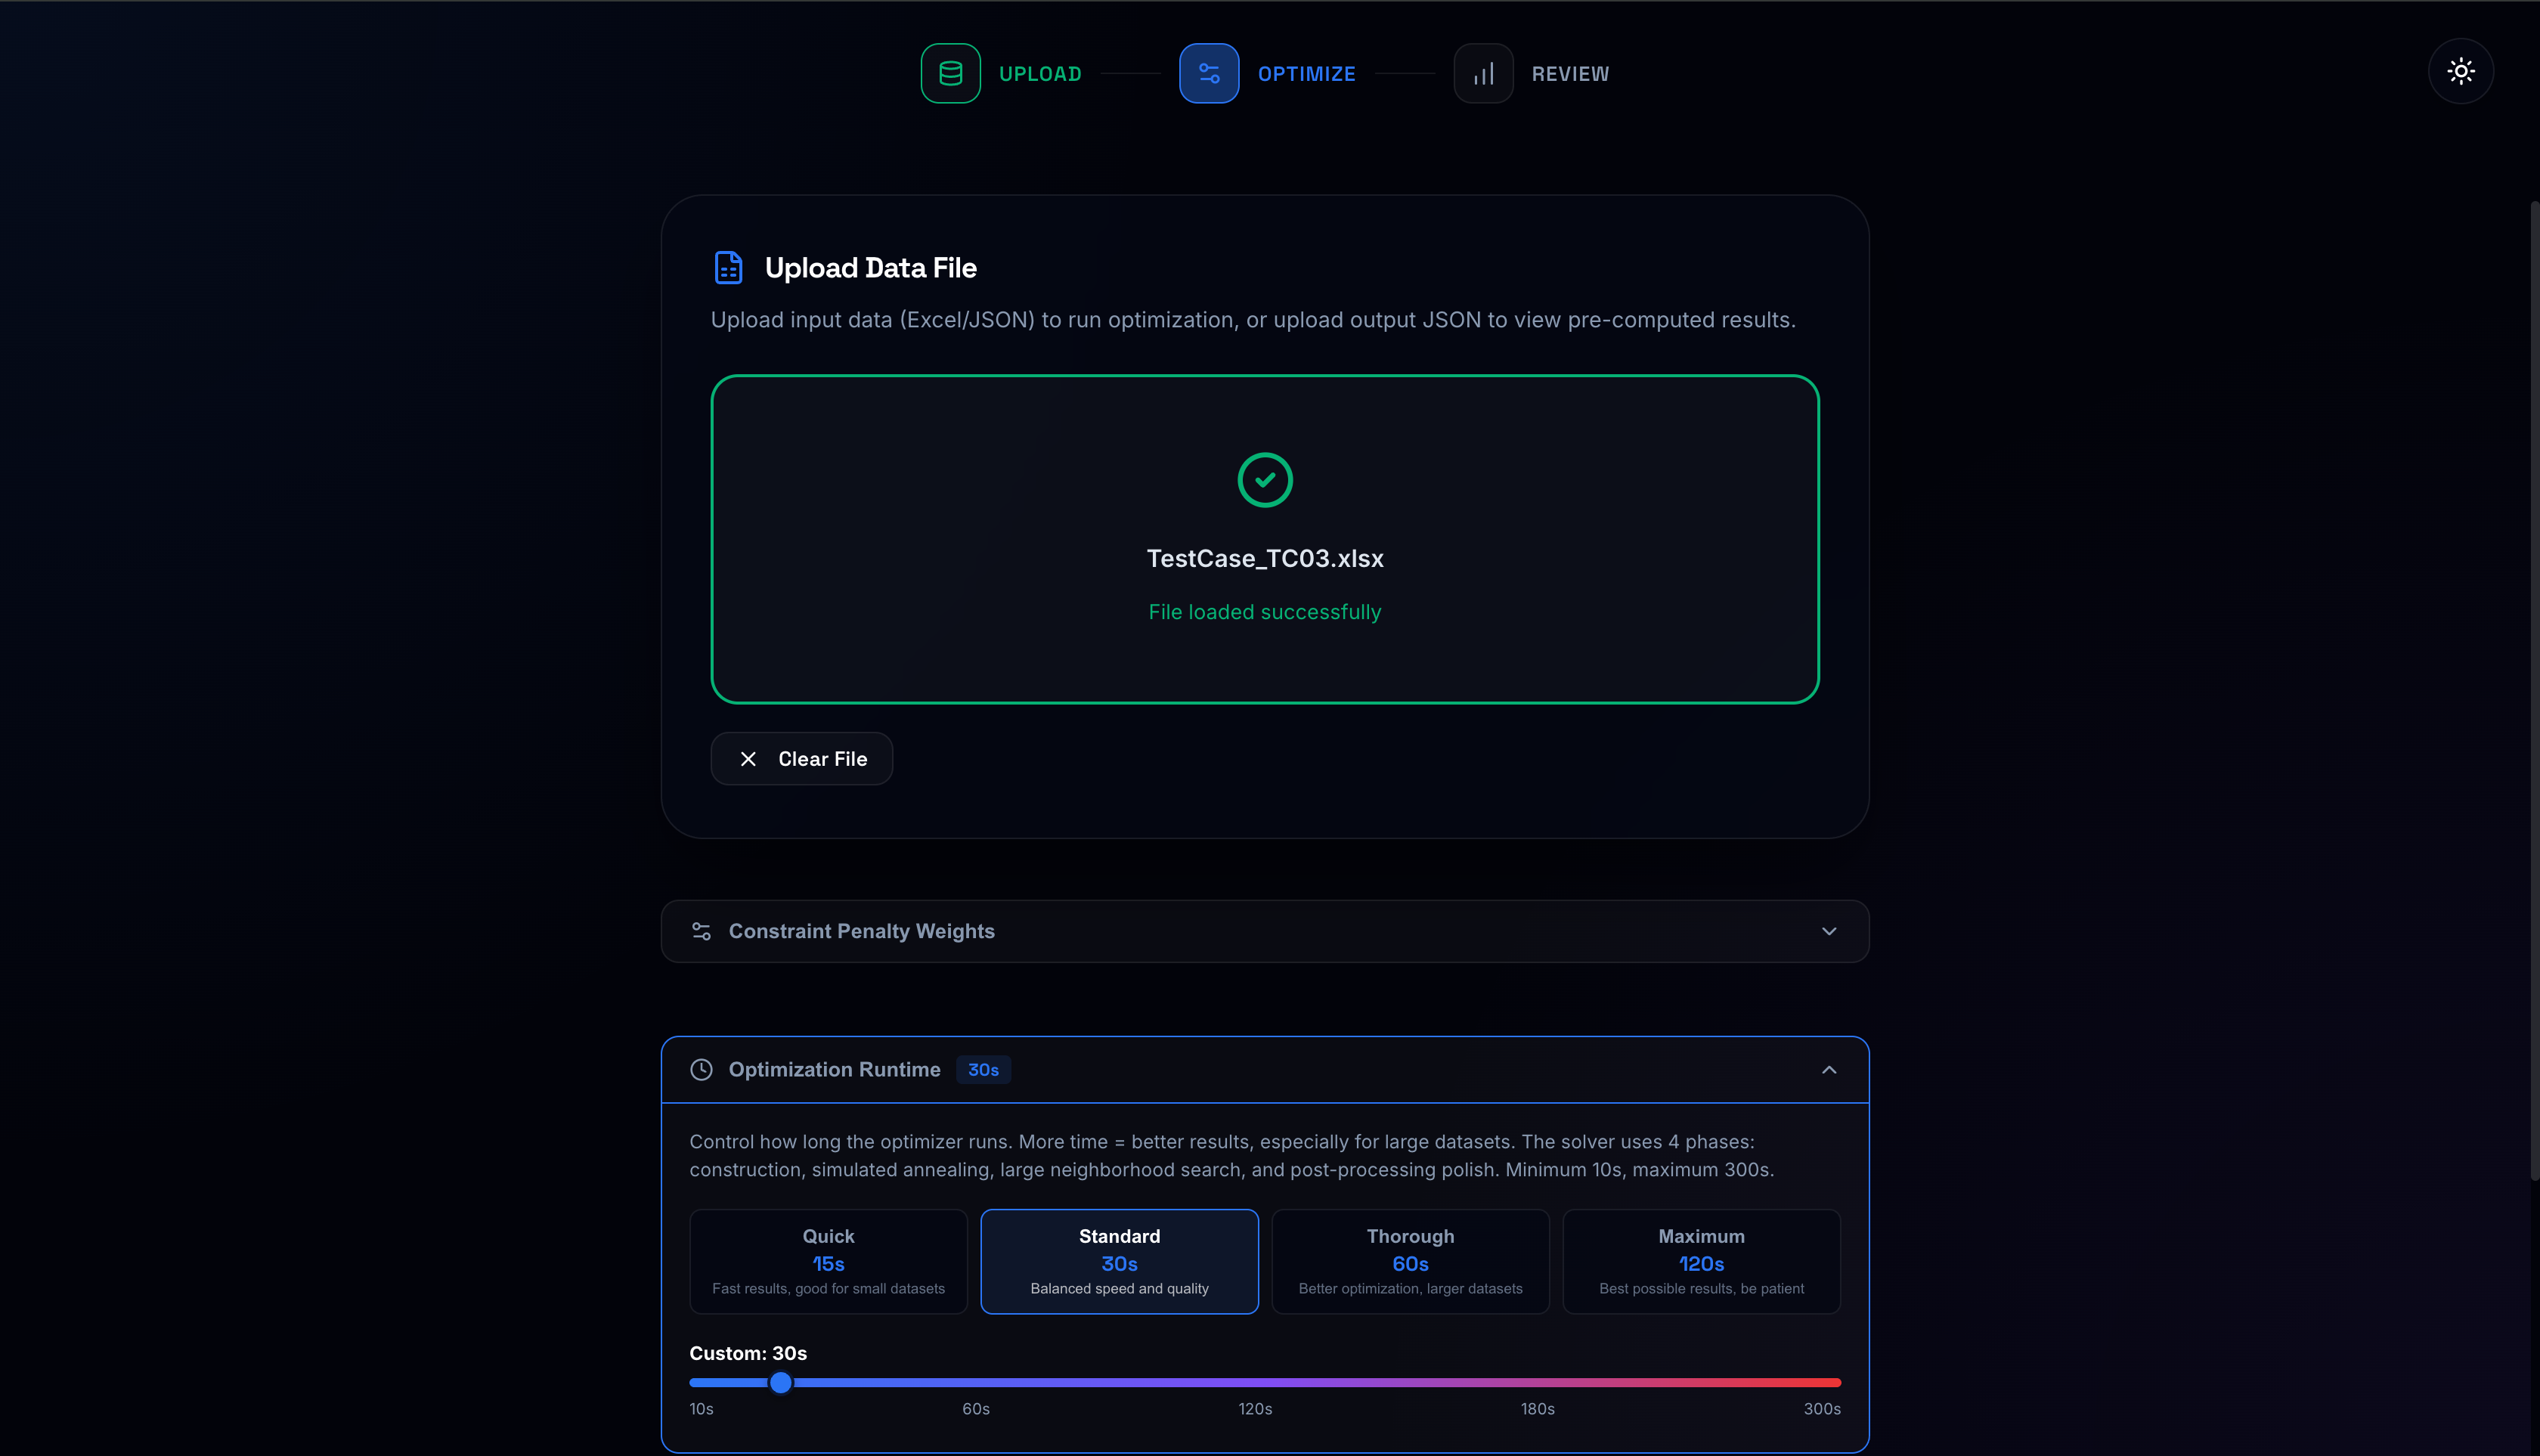
\includegraphics[width=0.494\linewidth]{Pic1.png}}%
\hspace{0.012\linewidth}%
\subcaptionbox{Employee results view\label{fig:ui-employees}}{%
  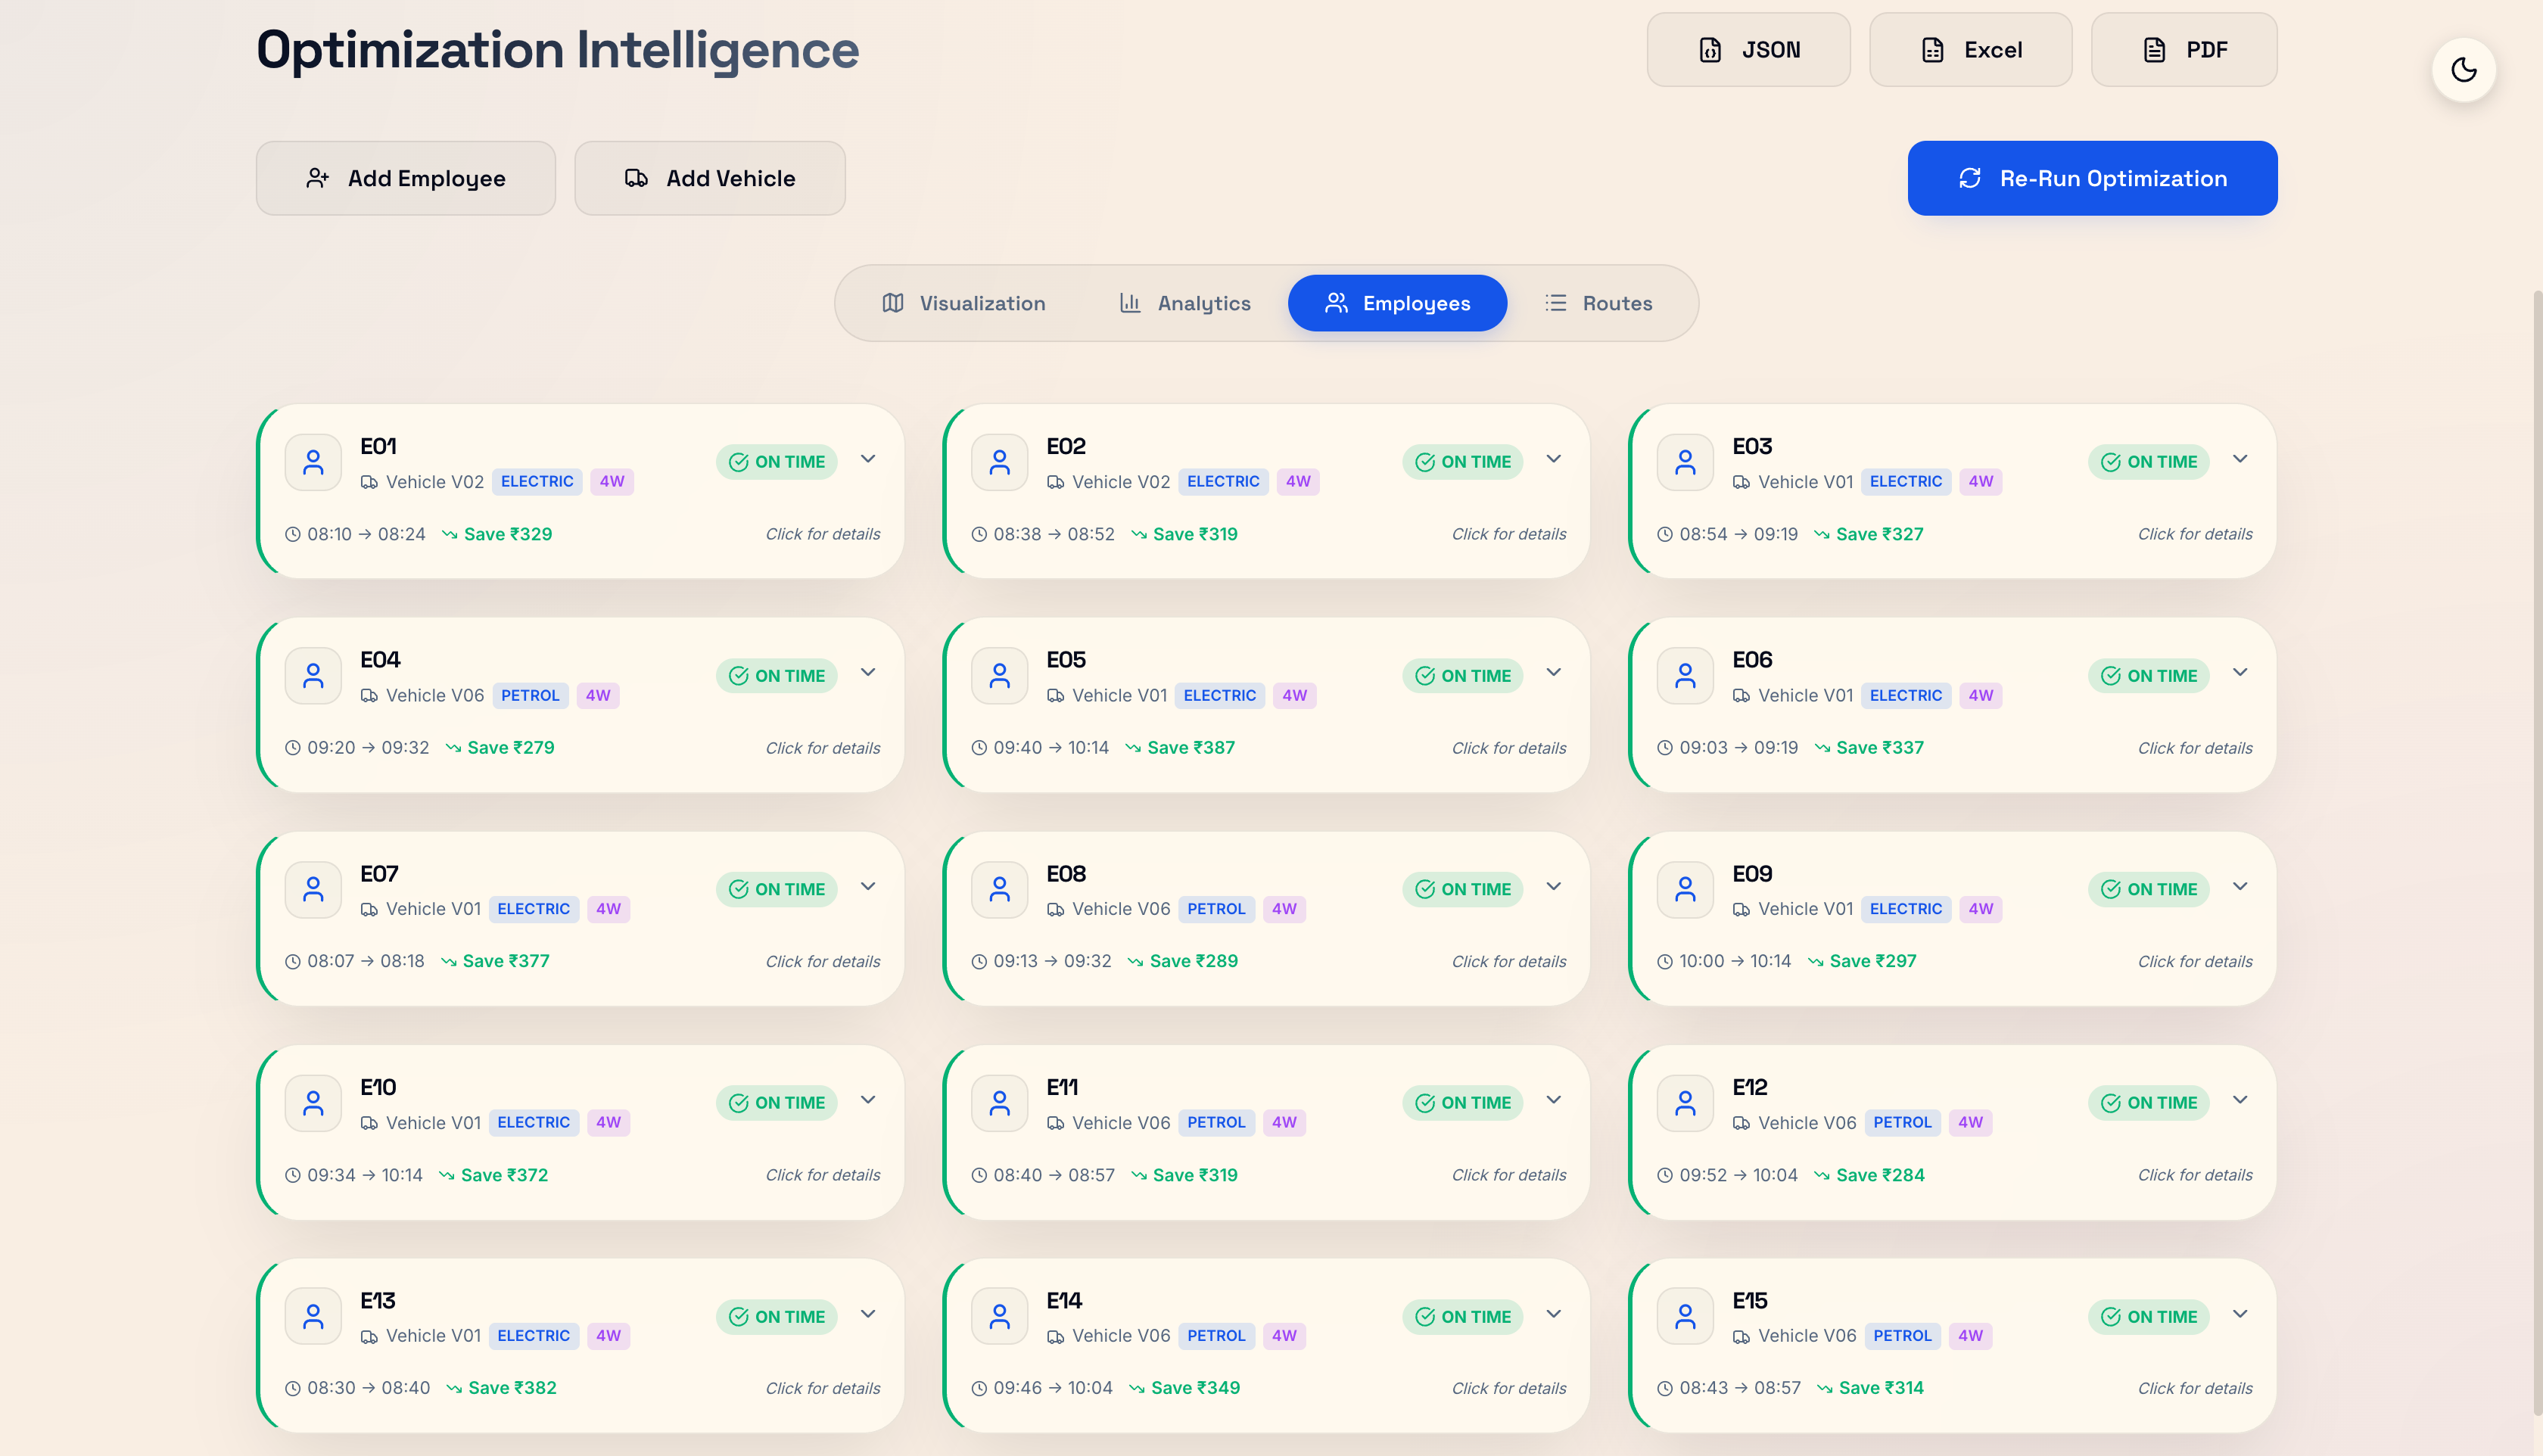
\includegraphics[width=0.494\linewidth]{Pic3.png}}}
\caption{Frontend screens used for input submission and results review.}
\label{fig:frontend-overview}
\end{figure}

\FloatBarrier

% ============================================================
% SECTION 4: ALGORITHM DESIGN
% ============================================================
\section{Algorithm Design}

The implemented search procedure operates on a route-state
\[
S = (R_1,\dots,R_{|K|},U),
\]
where each $R_k$ is an ordered route for vehicle $k$ and $U$ is the set of currently unserved requests. Every candidate state is evaluated through
\[
F(S)=w_c C(S)+w_t T(S)+\lambda_{\ell}L(S)+\lambda_s S_{\mathrm{share}}(S)+\lambda_p P_{\mathrm{pref}}(S)+\lambda_u |U|,
\]
which is the route-level realization of the objective in \cref{eq:objective-full}. The solver uses a \textbf{4-phase hybrid metaheuristic}: constructive initialization, Simulated Annealing improvement, ALNS diversification, and a final SA polish. The design follows Solomon-style insertion \cite{solomon1987}, Metropolis acceptance \cite{kirkpatrick1983}, and adaptive destroy-repair selection for ALNS \cite{ropke2006}.

% ---- Phase Pipeline Diagram ----
\vspace{6pt}
\begin{center}
\begin{tikzpicture}[
  node distance=0.38cm,
  box/.style={draw,rounded corners=4pt,minimum width=2.55cm,minimum height=0.85cm,
              font=\small\bfseries,align=center,inner sep=3pt},
  arr/.style={-{Stealth[length=5pt]},line width=1pt,color=velblue},
  lbl/.style={font=\scriptsize,color=veldark,align=center}
]
\node[box,fill=velblue!15,draw=velblue]   (p1) {Phase 1\\Construction};
\node[box,fill=velaccent!15,draw=velaccent,right=of p1] (p2) {Phase 2\\SA Warm-up};
\node[box,fill=velgreen!15,draw=velgreen,right=of p2]   (p3) {Phase 3\\ALNS};
\node[box,fill=velorange!15,draw=velorange,right=of p3] (p4) {Phase 4\\SA Polish};

\draw[arr] (p1)--(p2);
\draw[arr] (p2)--(p3);
\draw[arr] (p3)--(p4);

\node[lbl,below=0.12cm of p1] {Solomon I1\\up to 20 restarts};
\node[lbl,below=0.12cm of p2] {5 neighbourhoods\\Metropolis acceptance};
\node[lbl,below=0.12cm of p3] {adaptive\\destroy+repair};
\node[lbl,below=0.12cm of p4] {local\\intensification};
\end{tikzpicture}
\end{center}

\vspace{4pt}

\begin{figure}[htbp]
\centering
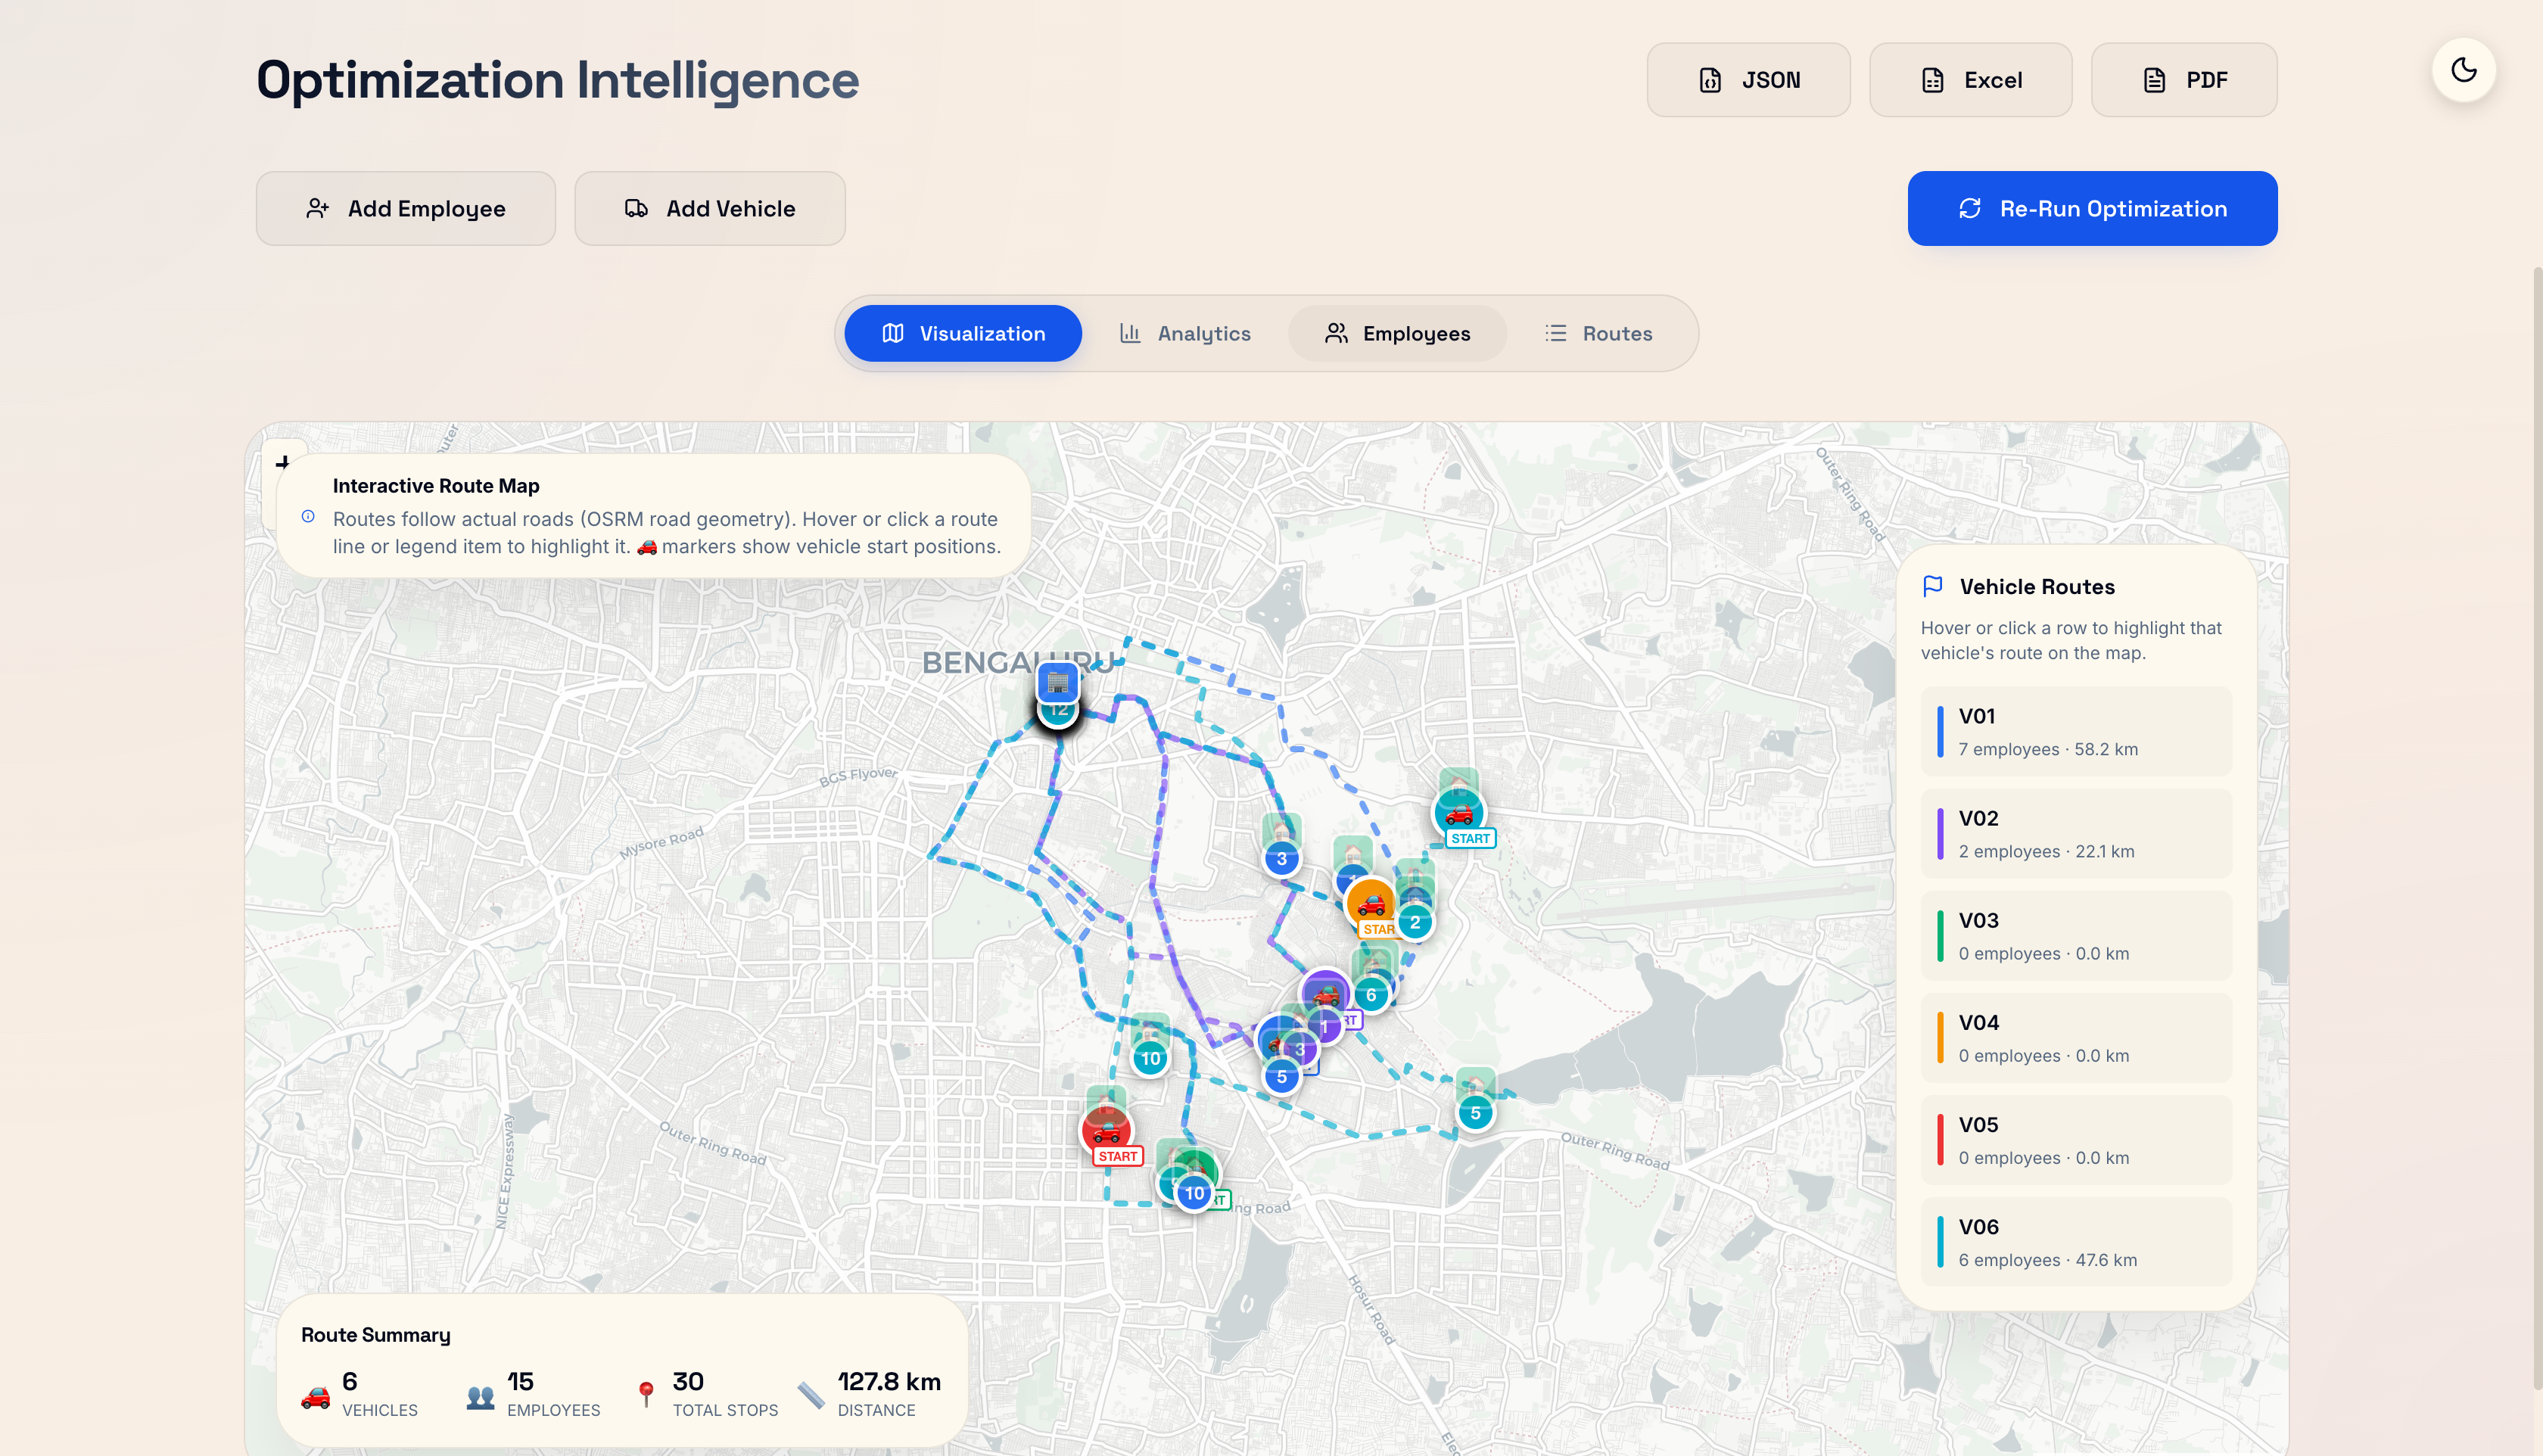
\includegraphics[width=0.72\linewidth]{Pic2.png}
\caption{Representative optimized routing output rendered on OSRM road geometry.}
\label{fig:solver-route-map}
\end{figure}

\noindent Figure~\ref{fig:solver-route-map} shows the type of route geometry inspected after optimization. The visualization is used to verify sequence quality, route overlap, and whether large detours match the final assignment logic.

\subsection{Phase 1 --- Solomon I1 Greedy Construction}

Phase 1 builds an initial incumbent $S_0$ through repeated Solomon-style insertion. Up to $\min(20,\lfloor 100/\bar{s}\rfloor)$ restarts are executed, where $\bar{s}$ is the average number of planned stops per vehicle. In each restart:
\begin{enumerate}[leftmargin=18pt,itemsep=1pt]
  \item \textbf{Shuffles} requests within priority buckets (P1 first, P5 last).
  \item For each unassigned request, evaluates the \textbf{cheapest feasible insertion position} across all vehicles and all positions in existing routes.
  \item Inserts the request if cost-increase is below a feasibility threshold; otherwise defers to force-assign.
\end{enumerate}
For request $i$, vehicle $k$, and insertion position $p$, the construction score is
\[
\Delta_{\mathrm{ins}}(i,k,p)=F\!\left(S\oplus(i,k,p)\right)-F(S),
\]
and the greedy move chooses the feasible triplet with minimum $\Delta_{\mathrm{ins}}$. The best solution among all restarts becomes the initial incumbent
\[
S_0 = \arg\min_{r\in\mathcal{R}} F\!\left(S^{(r)}\right).
\]

\noindent\textbf{Restart rationale.} The construction phase is order-sensitive, so shuffling within priority buckets adds diversity without violating service-level ordering.

\subsection{Phase 2 --- Simulated Annealing (SA)}

Phase 2 performs trajectory-based local search on the state space around $S_0$. At iteration $r$, the algorithm selects one of five neighbourhood operators, generates a candidate $S_r'$, computes
\[
\Delta_r = F(S_r') - F(S_r),
\]
and applies the Metropolis acceptance rule
\begin{equation}
S_{r+1} =
\begin{cases}
S_r', & \text{if }\Delta_r \le 0,\\
S_r', & \text{if }u_r < \exp(-\Delta_r/T_r),\quad u_r\sim \mathcal U(0,1),\\
S_r, & \text{otherwise.}
\end{cases}
\label{eq:sa-accept}
\end{equation}
Worse moves can still be accepted with temperature-controlled probability, which helps the search escape local minima early.

\vspace{4pt}
\begin{center}
\small
\begin{tabular}{@{}p{0.24\textwidth}cp{0.55\textwidth}@{}}
\toprule
\rowcolor{rowhead}\color{white}\textbf{Operator} & \color{white}\textbf{Weight} & \color{white}\textbf{Description}\\
\midrule
\rowcolor{rowalt}Greedy Relocate   & 28\% & Move request to cheapest feasible insertion across all vehicles\\
Intra-Route Relocate              & 28\% & Best re-insertion within same route\\
\rowcolor{rowalt}Exchange          & 18\% & Swap two requests between different routes\\
2-Opt                             & 13\% & Reverse a segment within a route\\
\rowcolor{rowalt}Or-Opt            & 13\% & Move a chain of 1--2 consecutive stops to another position\\
\bottomrule
\end{tabular}
\end{center}

\vspace{6pt}
\noindent\textbf{Temperature schedule.} Let $Z_0=F(S_0)$ and let $s$ denote the average route length. The first SA pass uses
\[
T_0 = \min(0.3 \times Z_0,\; 1000), \qquad
\alpha = 0.99, \qquad
\text{maxNoImprove} = \max\!\left(100,\, \frac{2000}{s}\right)
\]
with cooling law
\[
T_{r+1}=\alpha T_r .
\]
If the incumbent remains unchanged for a prolonged interval, the implementation reheats the search by multiplying the current temperature by $3.0$. This restores exploration without discarding the incumbent.

\subsection{Phase 3 --- Adaptive Large Neighbourhood Search (ALNS)}

Phase 3 broadens the search by alternating between \emph{destroy} and \emph{repair}. Starting from the best SA solution, ALNS partially dismantles the incumbent, rebuilds it, and updates operator preferences based on observed utility. Let
\[
\mathcal D=\{d_1,d_2,d_3\}, \qquad \mathcal R=\{r_1\},
\]
denote the sets of destroy and repair operators. At ALNS iteration $m$, an operator pair $(d,r)$ is drawn from probability distributions induced by adaptive weights, a partial state $\widetilde S_m=d(S_m)$ is created, and then a repaired candidate $S_m'=r(\widetilde S_m)$ is evaluated.

\vspace{4pt}
\begin{tcolorbox}[colback=velred!5, colframe=velred!50, title=Destroy Operators, fonttitle=\small\bfseries, boxrule=0.5pt, arc=2pt, top=4pt, bottom=4pt, left=6pt, right=6pt]
\small
\begin{itemize}[leftmargin=12pt,itemsep=2pt]
  \item \textbf{Shaw Removal:} remove a geographically related cluster of requests --- an anchor request plus its $k$ nearest neighbours by road distance.
  \item \textbf{Random Removal:} uniform random selection for diversification, prevents getting stuck.
  \item \textbf{Route Removal:} evict all requests from the highest-penalty route; forces radical restructuring to escape plateaus.
\end{itemize}
\end{tcolorbox}

\vspace{4pt}
\begin{tcolorbox}[colback=velgreen!5, colframe=velgreen!50, title=Repair Operator, fonttitle=\small\bfseries, boxrule=0.5pt, arc=2pt, top=4pt, bottom=4pt, left=6pt, right=6pt]
\small
\textbf{Regret-2 Insertion:} for each unassigned request compute:
\[
\mathrm{regret}_i = c_i^{(2)} - c_i^{(1)}
\]
Insert the request with \textit{highest regret} first. This prioritizes requests that are hardest to place later.
\end{tcolorbox}

\vspace{6pt}
\noindent\textbf{Repair logic.} The regret-based repair stage ranks unassigned requests by the loss incurred if the best insertion opportunity is skipped. If $\Delta_i^{(1)}$ and $\Delta_i^{(2)}$ are the best and second-best insertion costs for request $i$, then
\[
\mathrm{regret}_i = \Delta_i^{(2)} - \Delta_i^{(1)},
\]
and ALNS inserts the request with largest $\mathrm{regret}_i$ first. This prioritizes requests with few good insertion options.

\noindent\textbf{Adaptive operator update.} After candidate evaluation, each operator score is updated according to \cite{ropke2006}:
\[
w_o^{(m+1)} \leftarrow \lambda w_o^{(m)} + (1-\lambda)\sigma_o^{(m)},
\qquad \lambda=0.8,
\]
where $\sigma_o^{(m)} \in \{33,9,3,0\}$ for a new global best, an improved incumbent, an accepted non-improving move, and a rejected move, respectively. The normalized operator-selection probabilities are then
\[
\pi_o^{(m+1)}=\frac{w_o^{(m+1)}}{\sum_{o'} w_{o'}^{(m+1)}}.
\]
Candidate acceptance inside ALNS again follows a Metropolis criterion,
\[
\Pr(\text{accept }S_m')=
\begin{cases}
1, & F(S_m')\le F(S_m),\\
\exp\!\left(-\dfrac{F(S_m')-F(S_m)}{T_m^{\mathrm{ALNS}}}\right), & F(S_m')>F(S_m),
\end{cases}
\]
with a slower cooling factor $\alpha=0.998$. Relative to Phase 2, ALNS accepts larger structural changes while using the same global cost function.

\subsection{Phase 4 --- Post-ALNS SA Polish}

The final phase is a second SA pass initialized at the best ALNS incumbent. Its role is to clean up local inefficiencies after ALNS makes larger route-structure changes. If $S_{\mathrm{ALNS}}$ is the best solution after Phase 3 and $S_{\mathrm{P4}}$ is the result of the polish pass, the solver returns
\[
S^\star = \arg\min \left\{F(S_{\mathrm{ALNS}}),\; F(S_{\mathrm{P4}})\right\}.
\]
This final comparison ensures the best incumbent is preserved.

% ============================================================
% SECTION 5: TEST CASE RESULTS (TC01--TC03)
% ============================================================
\section{Test Case Results: TC01 -- TC03}

\noindent Each testcase is evaluated under three exported scenario runs. For compactness, the same scenario labels are reused across TC01--TC03.

\begin{center}\small
\begin{tabularx}{0.96\textwidth}{@{}p{0.10\textwidth}X@{}}
\toprule
\rowcolor{tblhead}\textbf{Label} & \textbf{Scenario} \\
\midrule
\rowcolor{rowalt}S1 & With Haversine, With Force Assigned ON, Without any Soft Constraint Penalty Weights \\
S2 & Using Real Map, With Force Assigned ON, Without any Soft Constraint Penalty Weights \\
\rowcolor{rowalt}S3 & Using Real Map, With Force Assigned ON, With Soft Constraint Penalty Weights \\
\bottomrule
\end{tabularx}
\end{center}

\subsection{TC01}

\begin{center}
\small
\renewcommand{\arraystretch}{1.34}
\setlength{\tabcolsep}{10pt}
\begin{tabular*}{0.99\textwidth}{@{\extracolsep{\fill}}lrrrrrr@{}}
\toprule
\rowcolor{tblhead}
\textbf{Scenario} & \textbf{CTC} & \textbf{Baseline} & \textbf{Optimization} & \textbf{Fleet} & \textbf{Distance} & \textbf{Time} \\
\midrule
\rowcolor{rowalt}S1 & \rupee571.30 & \rupee3,200.00 & 82.1\% & 2 / 3 & 48.56 km & 212 min \\
S2 & \rupee503.82 & \rupee3,200.00 & 84.3\% & 1 / 3 & 50.38 km & 136 min \\
\rowcolor{rowalt}S3 & \rupee802.00 & \rupee3,200.00 & 74.9\% & 2 / 3 & 68.13 km & 235 min \\
\bottomrule
\end{tabular*}
\captionof{table}{TC01 across the three requested scenarios.}
\label{tab:tc01-scenarios}
\end{center}

\noindent\textit{Reading.} TC01 achieves the highest optimization in S2 at \textbf{84.3\%}. The real-map run with soft penalties ON (S3) is costlier and uses more travel because the solution is less aggressively compressed.

\begin{center}
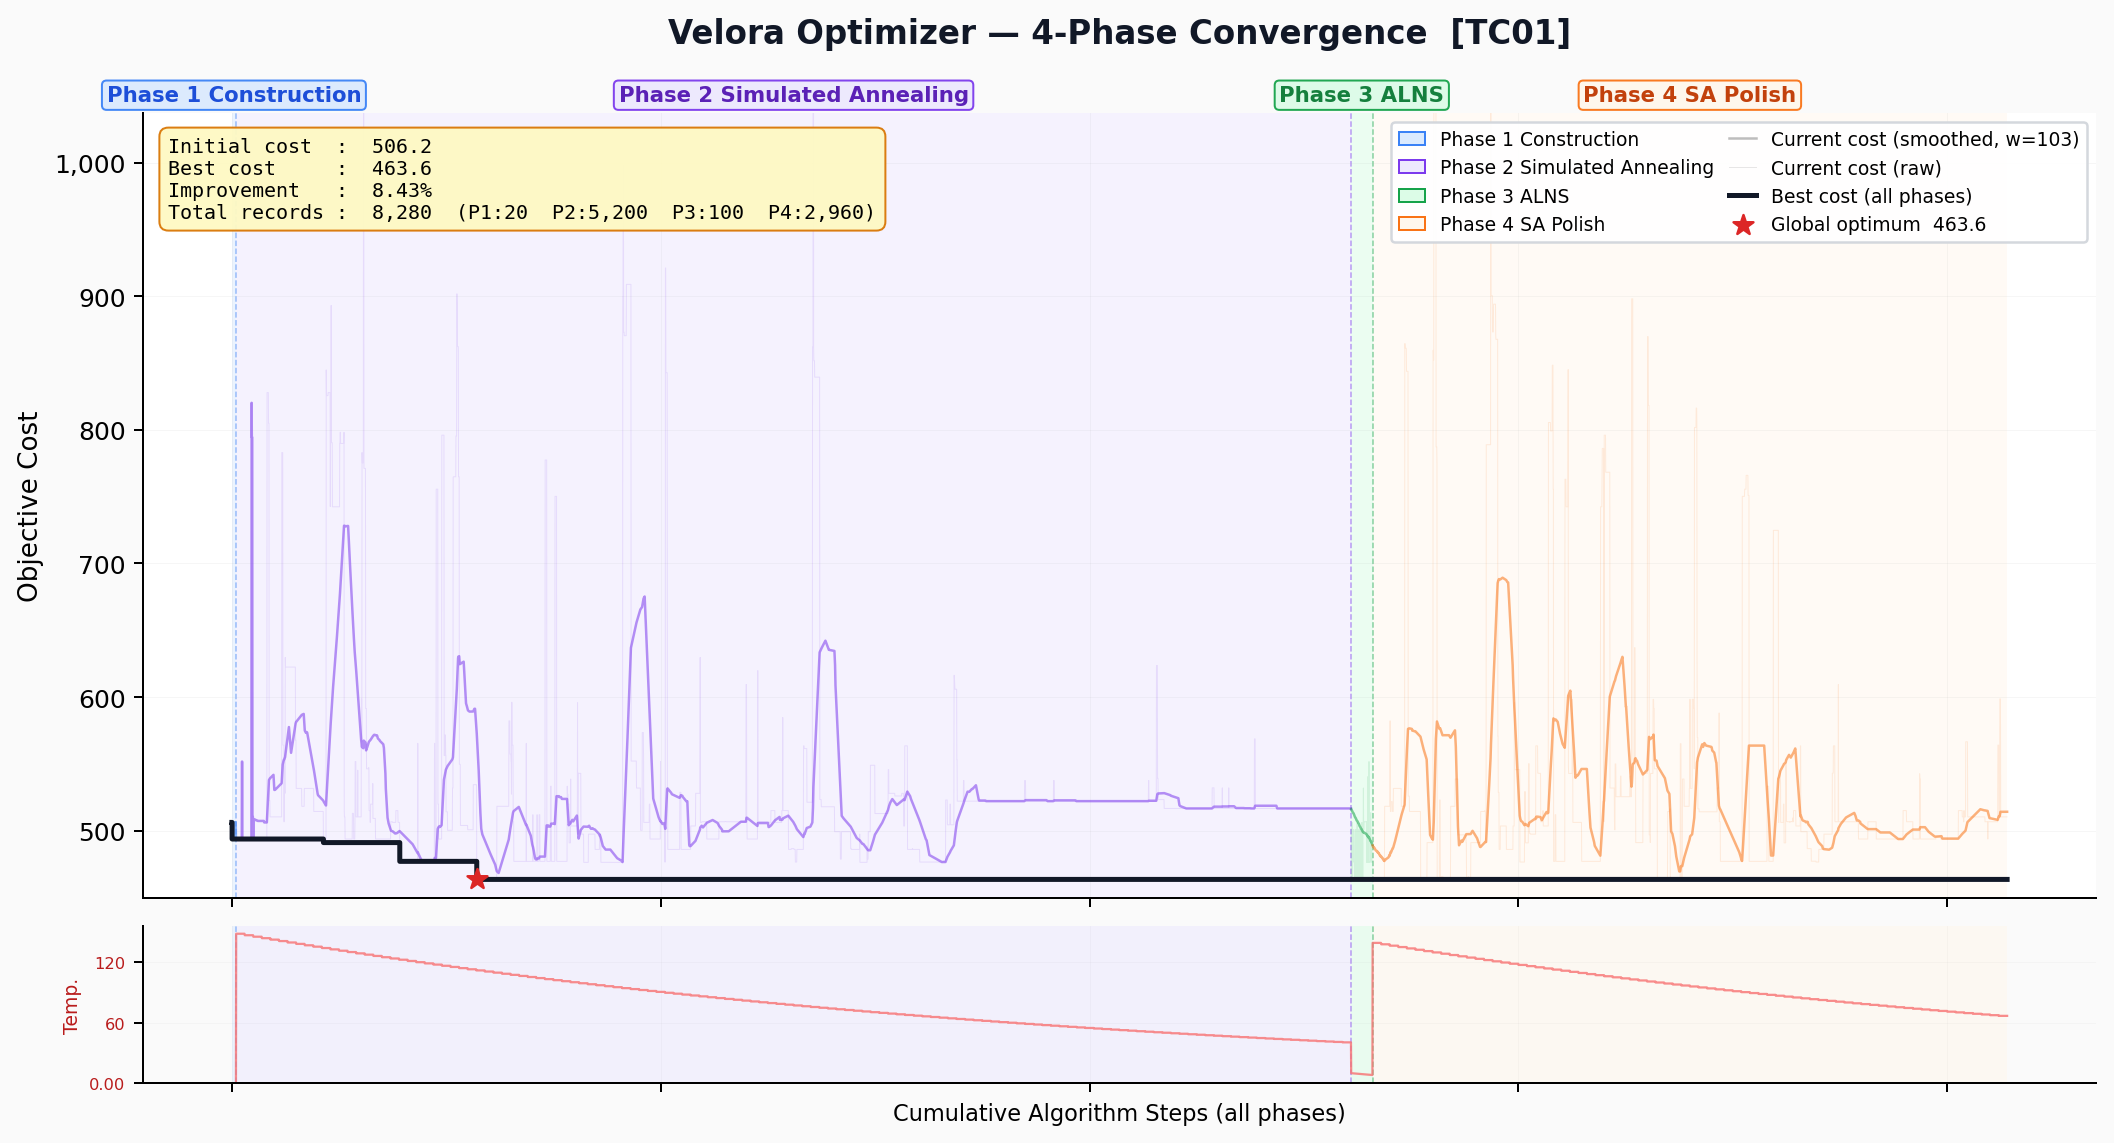
\includegraphics[width=0.90\linewidth]{tc01_convergence.png}
\captionof{figure}{TC01 convergence trace.}
\label{fig:tc01-convergence}
\end{center}

\noindent\textit{Convergence.} The cost falls quickly in the early iterations and then stabilizes. This indicates that the smallest testcase reaches a good route structure fast and needs only limited late-stage refinement.

\subsection{TC02}

\begin{center}
\small
\renewcommand{\arraystretch}{1.34}
\setlength{\tabcolsep}{10pt}
\begin{tabular*}{0.99\textwidth}{@{\extracolsep{\fill}}lrrrrrr@{}}
\toprule
\rowcolor{tblhead}
\textbf{Scenario} & \textbf{CTC} & \textbf{Baseline} & \textbf{Optimization} & \textbf{Fleet} & \textbf{Distance} & \textbf{Time} \\
\midrule
\rowcolor{rowalt}S1 & \rupee820.13 & \rupee4,945.00 & 83.4\% & 3 / 5 & 86.45 km & 274 min \\
S2 & \rupee692.09 & \rupee4,945.00 & 86.0\% & 2 / 5 & 67.64 km & 195 min \\
\rowcolor{rowalt}S3 & \rupee1,105.49 & \rupee4,945.00 & 77.6\% & 4 / 5 & 115.19 km & 344 min \\
\bottomrule
\end{tabular*}
\captionof{table}{TC02 across the three requested scenarios.}
\label{tab:tc02-scenarios}
\end{center}

\noindent\textit{Reading.} TC02 again performs best in S2, reaching \textbf{86.0\%} optimization. Once soft penalties are activated in S3, both CTC and fleet usage increase because the solver avoids the more aggressive consolidations allowed in S1--S2.

\begin{center}
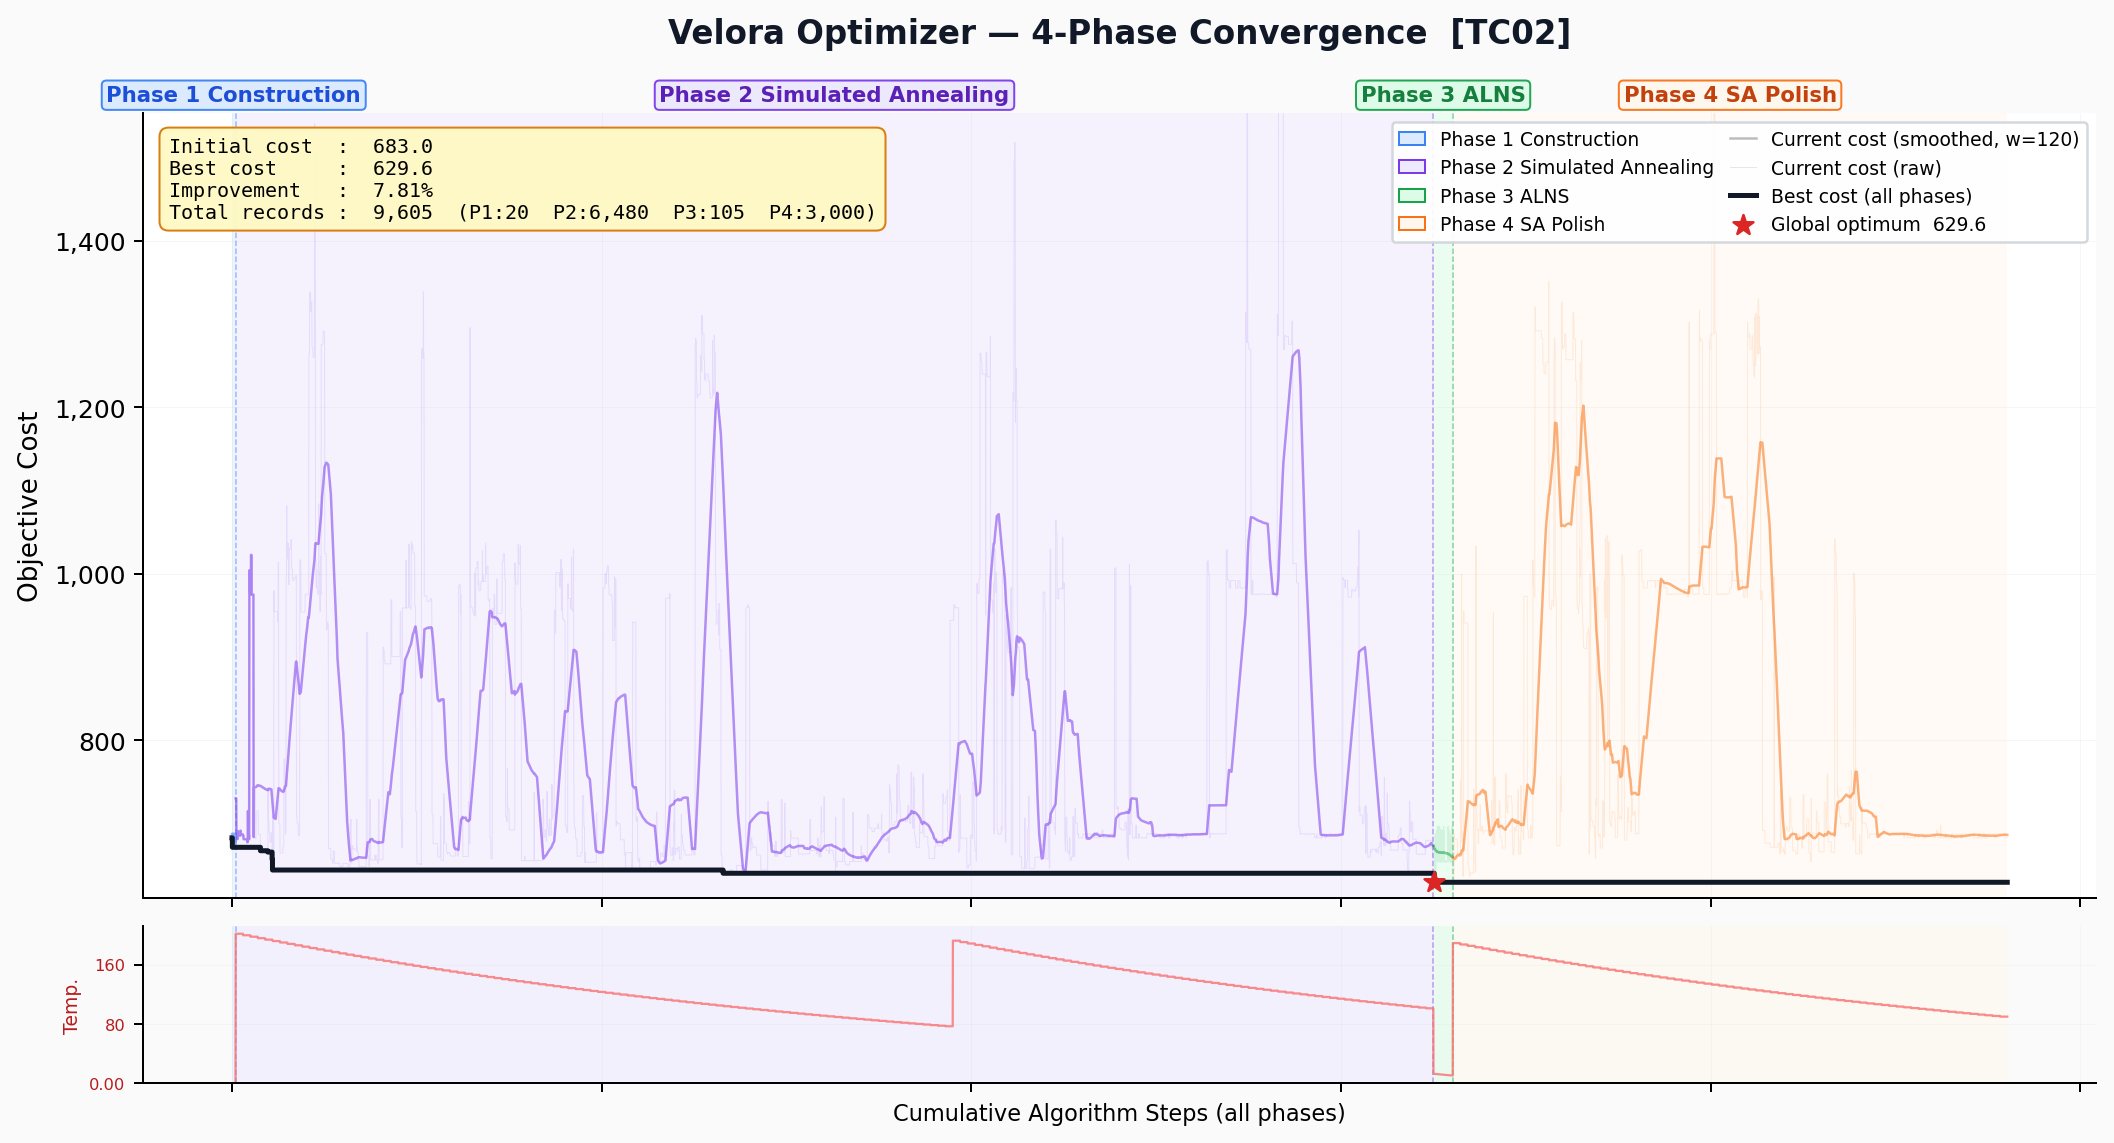
\includegraphics[width=0.90\linewidth]{tc02_convergence.png}
\captionof{figure}{TC02 convergence trace.}
\label{fig:tc02-convergence}
\end{center}

\noindent\textit{Convergence.} The best-cost curve still drops early, but the middle portion improves in clearer steps than TC01. This reflects a larger search space and more route interactions before the solver settles.

\subsection{TC03}

\begin{center}
\small
\renewcommand{\arraystretch}{1.34}
\setlength{\tabcolsep}{10pt}
\begin{tabular*}{0.99\textwidth}{@{\extracolsep{\fill}}lrrrrrr@{}}
\toprule
\rowcolor{tblhead}
\textbf{Scenario} & \textbf{CTC} & \textbf{Baseline} & \textbf{Optimization} & \textbf{Fleet} & \textbf{Distance} & \textbf{Time} \\
\midrule
\rowcolor{rowalt}S1 & \rupee933.57 & \rupee6,450.00 & 85.5\% & 4 / 6 & 94.10 km & 276 min \\
S2 & \rupee732.34 & \rupee6,450.00 & 88.6\% & 3 / 6 & 68.80 km & 244 min \\
\rowcolor{rowalt}S3 & \rupee1,331.87 & \rupee6,450.00 & 79.4\% & 4 / 6 & 129.02 km & 390 min \\
\bottomrule
\end{tabular*}
\captionof{table}{TC03 across the three requested scenarios.}
\label{tab:tc03-scenarios}
\end{center}

\noindent\textit{Reading.} TC03 shows the same pattern most clearly: S2 gives the highest optimization at \textbf{88.6\%}, while S3 trades cost for more service-aware routing. The soft-penalty-aware setting produces the longest routes and the highest travel time.

\begin{center}
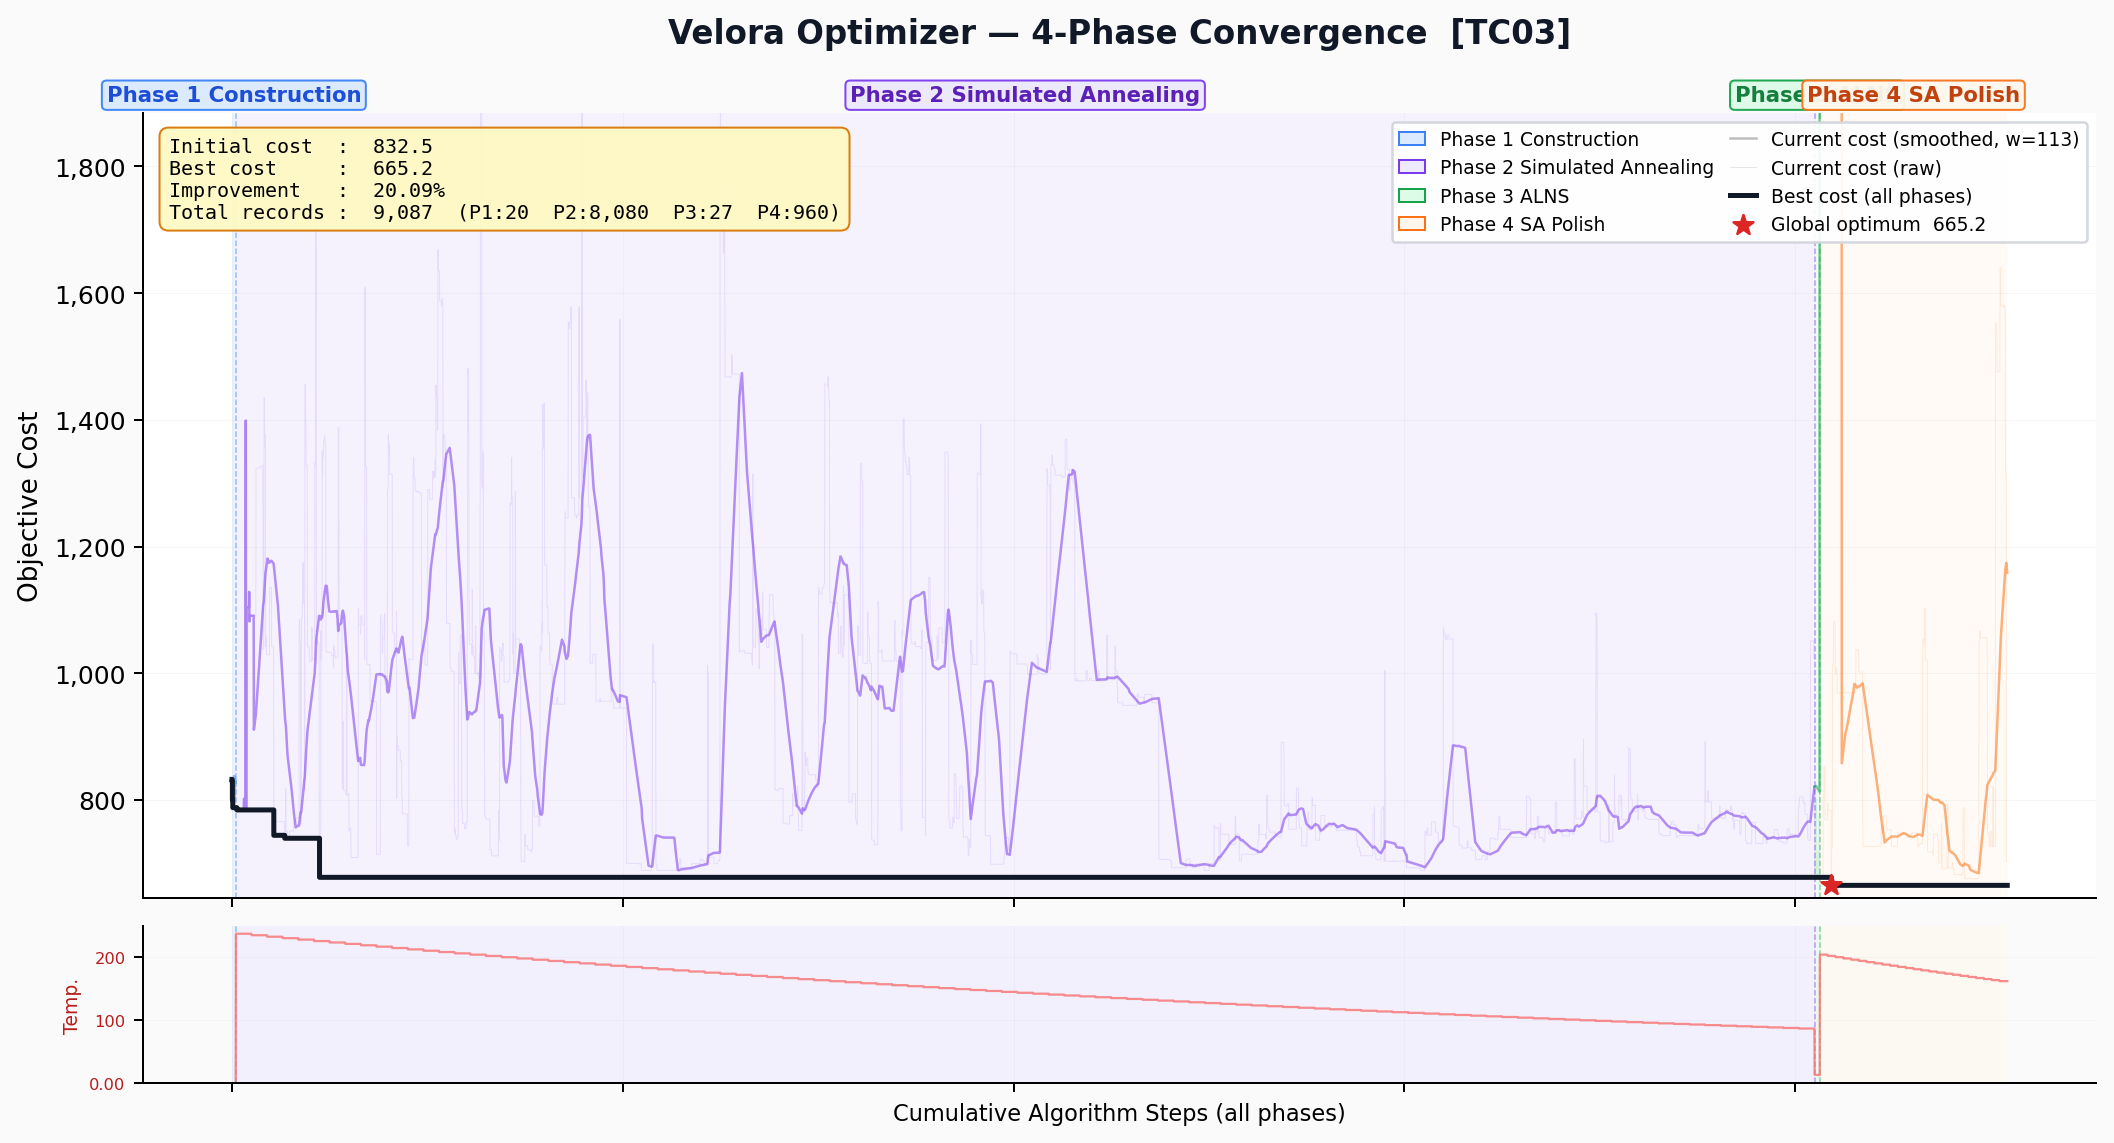
\includegraphics[width=0.90\linewidth]{tc03_convergence.png}
\captionof{figure}{TC03 convergence trace.}
\label{fig:tc03-convergence}
\end{center}

\noindent\textit{Convergence.} TC03 converges more gradually than TC01 and TC02. The larger instance and tighter routing trade-offs keep the search productive for longer before the curve flattens.


% ============================================================
  % SECTION 6: TC04 REDESIGNED ANALYSIS
  % ============================================================
\section{TC04 --- Penalty-Sensitive Stress Test}

\subsection{Scenario Overview}

\begin{center}
\footnotesize
\renewcommand{\arraystretch}{1.30}
\setlength{\tabcolsep}{5pt}
\begin{adjustbox}{width=\textwidth,center}
\begin{tabularx}{\textwidth}{@{}c c c c >{\raggedleft\arraybackslash}p{0.14\textwidth} >{\raggedleft\arraybackslash}p{0.10\textwidth} >{\raggedleft\arraybackslash}p{0.14\textwidth} X@{}}
\toprule
\rowcolor{tblhead}
\textbf{Cfg.} & \textbf{Map} & \textbf{Force} & \textbf{Soft} & \textbf{CTC} & \textbf{Savings} & \textbf{Penalty} & \textbf{Result summary}\\
\midrule
\rowcolor{rowalt}S1 & Hav.  & ON  & OFF & \rupee1,149.23 & 74.0\% & \rupee977,345.44 & Full assignment; E10 remains hard-infeasible.\\
S2 & Real & ON  & OFF & \rupee1,383.86 & 68.7\% & \rupee1,554,180.00 & Real-road travel exposes the infeasibility cost.\\
\rowcolor{rowalt}S3 & Real & ON  & ON  & \rupee1,846.94 & 58.2\% & \rupee1,554,557.53 & \textbf{Preferred configuration}; realistic and fully assigned.\\
S4 & Hav.  & OFF & OFF & \rupee462.46 & 89.5\% & \rupee50,000.00 & Cheapest transport plan, but E10 is unassigned.\\
\bottomrule
\end{tabularx}
\end{adjustbox}
\captionof{table}{TC04 summary across the four solver configurations.}
\end{center}

\noindent TC04 contains 10 employees and 4 vehicles, including five P1 requests that prefer premium vehicles and largely avoid sharing. The case is penalty-sensitive because one request is structurally infeasible even in the preferred full-assignment setting.

\begin{warnbox}[Structural Infeasibility]
\small
Employee \textbf{E10} starts about 33\,km from the office and has an 08:00--08:40 P1 window with only 5 minutes of tolerance. In the preferred real-map run, the achieved office arrival is still \textbf{09:47}. Any full-assignment solution therefore pays a large hard time-window penalty.
\end{warnbox}

\subsection{Scenario S2 --- Real Map, Force ON, Soft OFF}

Scenario S2 removes soft-constraint penalty weights while keeping real-road distance and full assignment. This isolates the effect of service-quality penalties from the structural E10 infeasibility.

\begin{center}
\small
\renewcommand{\arraystretch}{1.38}
\setlength{\tabcolsep}{9pt}
\begin{tabularx}{\textwidth}{@{} >{{\RaggedRight\arraybackslash}}X >{{\raggedleft\arraybackslash}}p{2.8cm} >{{\raggedleft\arraybackslash}}p{2.5cm} >{{\raggedleft\arraybackslash}}p{2cm} @{}}
\toprule
\rowcolor{tblhead}
\textbf{Metric} & \textbf{Optimized} & \textbf{Baseline} & \textbf{Savings}\\
\midrule
\rowcolor{rowalt}Transport cost & \rupee1,383.86 & \rupee4,420.00 & 68.7\%\\
Total travel time & 327 min & --- & ---\\
\rowcolor{rowalt}Vehicles used & 4 & 10 cabs & 60.0\% fewer\\
Penalty cost & \rupee1,554,180.00 & --- & ---\\
\rowcolor{rowalt}Global objective & \rupee1,555,246.92 & --- & ---\\
\bottomrule
\end{tabularx}
\captionof{table}{Scenario S2 overall metrics.}
\end{center}

\begin{center}
\small
\renewcommand{\arraystretch}{1.38}
\setlength{\tabcolsep}{8pt}
\begin{tabularx}{\textwidth}{@{}l c Y >{\raggedleft\arraybackslash}p{1.9cm} >{\raggedleft\arraybackslash}p{1.8cm} >{\RaggedRight\arraybackslash}p{1.85cm}@{}}
\toprule
\rowcolor{tblhead}
\textbf{Route} & \textbf{Veh.} & \textbf{Employees} & \textbf{Distance} & \textbf{Cost} & \textbf{Status}\\
\midrule
\rowcolor{rowalt}R1 & V01 & E09 & 14.2 km & \rupee142 & Feasible\\
R2 & V02 & E08, E07 & 10.6 km & \rupee117 & Feasible\\
\rowcolor{rowalt}R3 & V03 & E10 & 62.5 km & \rupee875 & E10 violated\\
R4 & V04 & E02, E01, E06, E05, E03, E04 & 13.9 km & \rupee250 & Feasible\\
\bottomrule
\end{tabularx}
\captionof{table}{Scenario S2 route breakdown.}
\end{center}

\noindent\textit{Reading.} S2 already pays the full hard penalty for E10, but it minimizes transport cost aggressively everywhere else. The cheapest move is to compress six employees into a single short V04 route and accept any service-quality degradation that would otherwise be penalized.

\subsection{Preferred Scenario S3}

Scenario S3 (\textbf{Real Map + Force ON + Soft ON}) is the preferred benchmark because it keeps full assignment, uses road-network distance, and preserves service-quality penalties.

\begin{center}
\small
\renewcommand{\arraystretch}{1.38}
\setlength{\tabcolsep}{9pt}
\begin{tabularx}{\textwidth}{@{} >{{\RaggedRight\arraybackslash}}X >{{\raggedleft\arraybackslash}}p{2.8cm} >{{\raggedleft\arraybackslash}}p{2.5cm} >{{\raggedleft\arraybackslash}}p{2cm} @{}}
\toprule
\rowcolor{tblhead}
\textbf{Metric} & \textbf{Optimized} & \textbf{Baseline} & \textbf{Savings}\\
\midrule
\rowcolor{rowalt}Transport cost & \rupee1,846.94 & \rupee4,420.00 & 58.2\%\\
Total travel time & 351 min & 485 min & 27.6\%\\
\rowcolor{rowalt}Vehicles used & 4 & 10 cabs & 60.0\% fewer\\
Penalty cost & \rupee1,554,557.53 & --- & ---\\
\rowcolor{rowalt}Global objective & \rupee1,555,955.70 & --- & ---\\
\bottomrule
\end{tabularx}
\captionof{table}{Scenario S3 overall metrics.}
\end{center}

\noindent\textit{Reading.} S3 still cuts direct transportation cost relative to the baseline, but the objective is dominated by E10's hard time-window violation.

\begin{center}
\small
\renewcommand{\arraystretch}{1.38}
\setlength{\tabcolsep}{8pt}
\begin{tabularx}{\textwidth}{@{}l c Y >{\raggedleft\arraybackslash}p{1.9cm} >{\raggedleft\arraybackslash}p{1.8cm} >{\RaggedRight\arraybackslash}p{1.85cm}@{}}
\toprule
\rowcolor{tblhead}
\textbf{Route} & \textbf{Veh.} & \textbf{Employees} & \textbf{Distance} & \textbf{Cost} & \textbf{Status}\\
\midrule
\rowcolor{rowalt}R1 & V01 & E01, E03, E05, E06, E09 & 57.6 km & \rupee576 & Feasible\\
R2 & V02 & E02, E04 & 21.9 km & \rupee241 & Feasible\\
\rowcolor{rowalt}R3 & V03 & E10 & 62.5 km & \rupee875 & E10 violated\\
R4 & V04 & E08, E07 & 8.6 km & \rupee155 & Feasible\\
\bottomrule
\end{tabularx}
\captionof{table}{Scenario S3 route breakdown.}
\end{center}

\begin{center}
\small
\renewcommand{\arraystretch}{1.38}
\setlength{\tabcolsep}{8pt}
\begin{tabularx}{\textwidth}{@{} >{{\RaggedRight\arraybackslash}}X >{{\centering\arraybackslash}}p{3.2cm} >{{\RaggedRight\arraybackslash}}p{5.1cm} @{}}
\toprule
\rowcolor{tblhead}
\textbf{Constraint component} & \textbf{Value} & \textbf{Reading}\\
\midrule
\rowcolor{rowalt}Hard time-window penalty & \rupee1,554,180.00 & Dominated by E10\\
Late-arrival penalty & \rupee77.53 & Minor residual delay\\
\rowcolor{rowalt}Vehicle-preference penalty & \rupee300.00 & E10 not served by premium vehicle\\
Sharing penalty & \rupee0.00 & No sharing violation\\
\bottomrule
\end{tabularx}
\captionof{table}{Scenario S3 penalty composition.}
\end{center}

\noindent Nine employees are served cleanly in S3. E10 is isolated on its own route, which prevents the infeasible request from degrading the rest of the schedule.

\subsection{Why S2 Has Lower CTC Than S3}

\noindent The CTC gap between S2 and S3 is primarily a routing-structure effect, not a change in the hard E10 infeasibility. In both scenarios, E10 remains the dominant hard time-window violation. The transport-cost difference arises because S2 is allowed to ignore soft service quality:

\begin{itemize}[leftmargin=16pt,itemsep=2pt]
  \item In \textbf{S2}, the solver can consolidate six employees into one very short V04 route costing only \rupee250.
  \item In \textbf{S3}, those requests are split across more routes to preserve better vehicle matching and service quality, so route cost rises even before penalties are added.
  \item \textbf{S2} does not pay for soft lateness or vehicle-preference violations, so it has no incentive to keep the same quality level as S3.
  \item The additional penalty terms in \textbf{S3} are relatively small compared with the hard E10 penalty; the larger practical difference is that soft penalties force a less compressed and more realistic route plan.
\end{itemize}

\noindent Qualitatively, S2 behaves like a transport-only optimizer once the structural E10 penalty is unavoidable: it minimizes fleet cost around that fixed hard violation. S3 behaves like a service-aware optimizer: it still cannot rescue E10, but it avoids degrading the remaining nine assignments just to save route cost.

\begin{center}
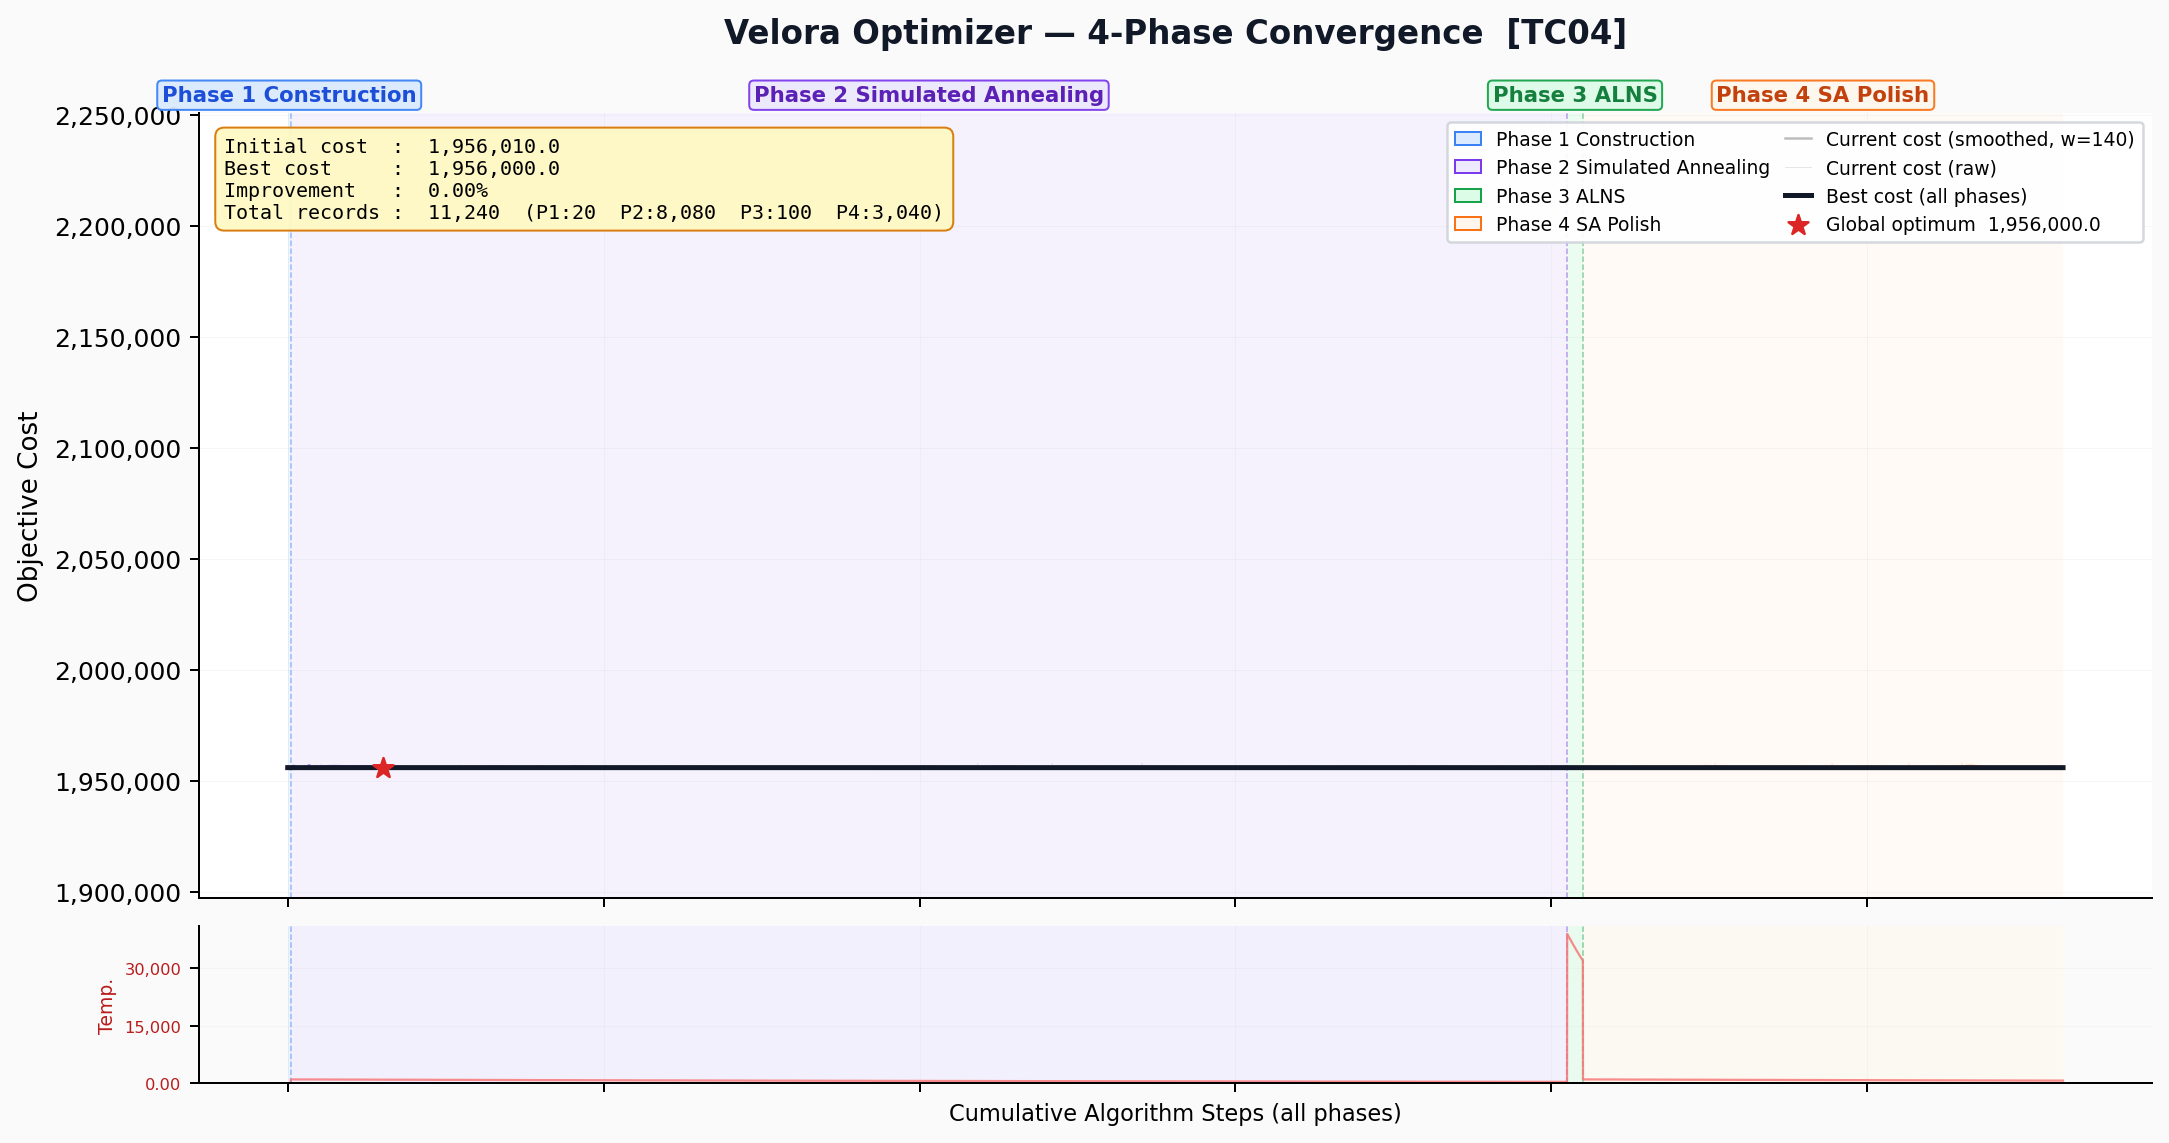
\includegraphics[width=0.90\linewidth]{tc04_convergence.png}
\captionof{figure}{TC04 convergence trace for Scenario S3.}
\label{fig:tc04-convergence}
\end{center}

\begin{insightbox}[TC04 Key Findings]
\small
\begin{enumerate}[leftmargin=18pt,itemsep=2pt]
  \item \textbf{S3 is the correct benchmark.} It preserves full assignment and keeps the service-quality terms active.
  \item \textbf{The dominant cost is structural, not routing noise.} E10 drives the hard time-window penalty.
  \item \textbf{The rest of the schedule is operationally clean.} Nine of ten employees are served without timing or sharing violations.
\end{enumerate}
\end{insightbox}
\par\medskip


\FloatBarrier

% ============================================================
% SECTION 7: HACK TEST CASE
% ============================================================
\section{Hack Test Case}
\label{sec:hack}

The retained adversarial case focuses on infeasibility detection, which is the most important robustness requirement for an employee-routing system.

\subsection{HC-01 --- Impossible Time Window}

\begin{hackbox}[HC-01 --- Impossible Time Window]
\small
\textbf{Input sheet:} \href{https://docs.google.com/spreadsheets/d/10i1GiT_c1rK27x5uJG4iGw2c_u7VGDNo/edit?gid=736445089#gid=736445089}{Google Sheet input}

\textbf{Output sheet:} \href{https://docs.google.com/spreadsheets/d/1cEbebLy069o2lC6KWmAdVSrs0sOf61_J/edit?gid=569214064#gid=569214064}{Google Sheet output}

\textbf{Test intent:} This case has employee pickup windows that do not overlap with any vehicle availability, making a feasible assignment impossible.

\textbf{Why it matters:}
\begin{itemize}[leftmargin=14pt,itemsep=1pt]
  \item Verifies whether the solver correctly detects infeasibility.
  \item Confirms that time-window constraints are not silently relaxed.
  \item Ensures the system reports invalid scheduling pressure instead of fabricating an unrealistic route plan.
\end{itemize}
\end{hackbox}

\begin{insightbox}[Why This Case Is Retained]
\small This is the cleanest robustness check in the report: it verifies that the optimizer detects an impossible schedule and reports it explicitly rather than fabricating a route.
\end{insightbox}

% ============================================================
% SECTION 8: RESOURCES
% ============================================================
\section{Resources}

\begin{center}\small
\begin{tabularx}{0.94\textwidth}{@{}p{0.24\textwidth}X@{}}
\toprule
\rowcolor{tblhead}\textbf{Resource} & \textbf{Link} \\
\midrule
\rowcolor{rowalt}Source code &
\href{https://github.com/bfea-kriti/VeloraMobilityOptimizer}{github.com/bfea-kriti/VeloraMobilityOptimizer} \\
Frontend deployment &
\href{https://velorafrontend-kri-2651-ti.onrender.com}{velorafrontend-kri-2651-ti.onrender.com} \\
\rowcolor{rowalt}Backend deployment &
\href{https://velorabackend-kri-2651-ti.onrender.com}{velorabackend-kri-2651-ti.onrender.com} \\
Demonstration video &
\href{https://www.youtube.com/watch?v=4BbK0500LLs}{youtube.com/watch?v=4BbK0500LLs} \\
\bottomrule
\end{tabularx}
\end{center}

% ============================================================
% SECTION 9: REFERENCES
% ============================================================
\FloatBarrier
\phantomsection
\addcontentsline{toc}{section}{References}
\bibliographystyle{plainnat}
\bibliography{references}

\end{document}
